%-----------------------------------------------------------------------------%
\chapter{\babEmpat}
%-----------------------------------------------------------------------------%

%-----------------------------------------------------------------------------%
\section{Implementasi Aplikasi}
%-----------------------------------------------------------------------------%

Implementasi aplikasi merupakan tahapan realisasi dari perancangan yang telah dibuat. Pada tahap ini akan dilakukan penjelasan mengenai antarmuka aplikasi “\textbf{SiPJabS: Sistem Pengawakan Jabatan Struktural di Universitas Telkom}”. 

\subsection{Implementasi Admin}

\begin{enumerate}
	
	\item Halaman \textit{Login}
	\begin{figure}
		\centering
		\includegraphics[width=0.8\textwidth]
		{pics/admin/implementasi/login.png}
		\caption{Halaman \textit{Login} Admin}
		\label{fig:CC10}
	\end{figure}

	Gambar tampilan diatas merupakan implementasi dari BAB III dimana admin harus menginputkan \textit{username} dan \textit{password} untuk dapat melanjutkan penggunaan aplikasi, apabila sudah diinput lanjut untuk mengklik \textit{button “login”}. 
	
	\newpage
	\item Halaman \textit{Dashboard}
	\begin{figure}
		\centering
		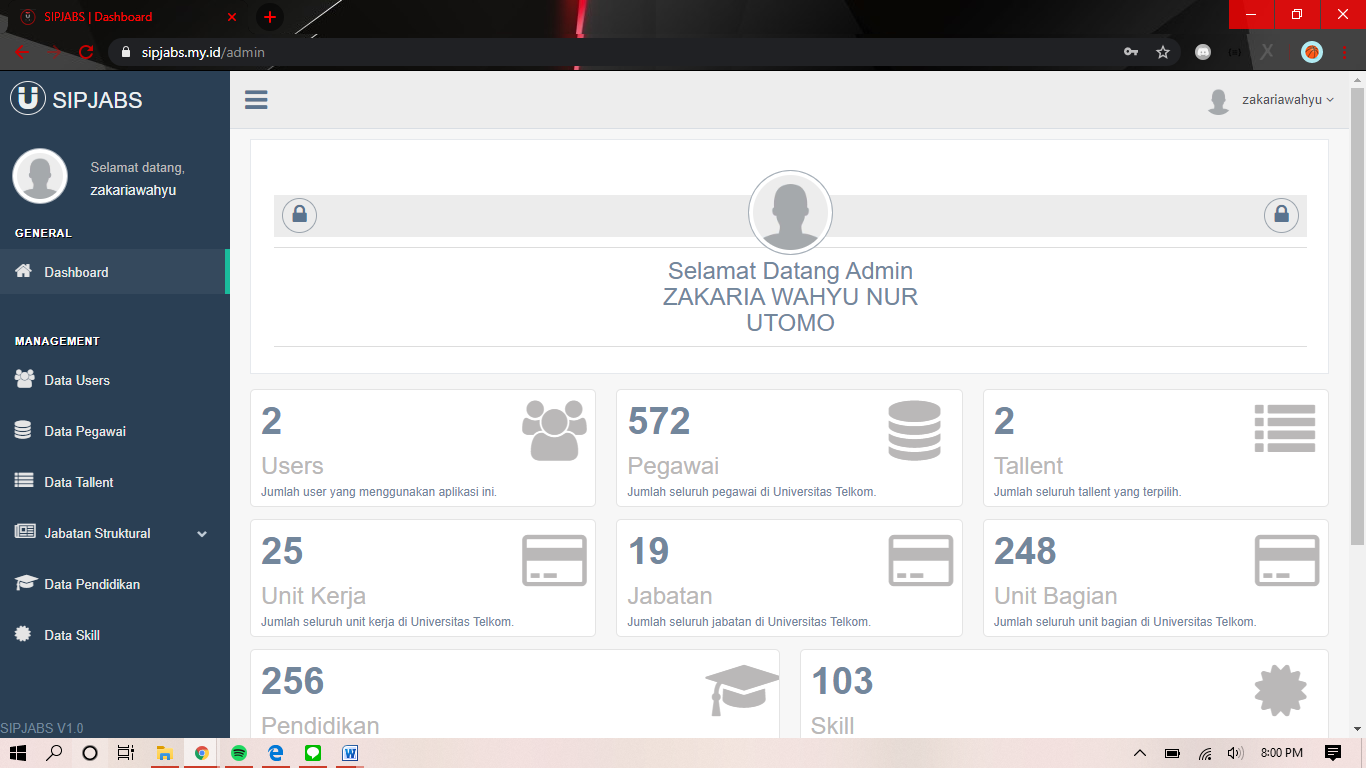
\includegraphics[width=0.8\textwidth]
		{pics/admin/implementasi/dashboard.png}
		\caption{Halaman \textit{Dashboard} Admin}
		\label{fig:CC10}
	\end{figure}
	Gambar diatas menjelaskan isi dari \textit{dashboard} admin, dibagi menjadi beberapa bagian diantaranya: terdapat jumlah \textit{user} yang dapat mengakses aplikasi SiPJabS sebagai admin maupun \textit{user}. Apabia admin menambahkan atau menghapus \textit{user} maka jumlah tersebut dapat berubah. Terdapat jumlah pegawai di Universitas Telkom. Kemudian jumlah \textit{tallent} yang sudah dipilih oleh user untuk menggantikan atau mengisi posisi yang kosong. Dibawahnya terdapat unit kerja yang didalamnya terdapat beberapa jabatan, dan didalam unit kerja juga dibagi menjadi unit bagian, agar pekerjaan lebih mudah untuk dikerjakan. Kemudian terdapat pendidikan yang dimiliki oleh pegawai Universitas Telkom, dan terakhir terdapat \textit{skill} yang dimiliki pegawai Universitas Telkom guna menunjang kerja.
	
	\newpage
	\item Halaman \textit{Profile}
	\begin{figure}
		\centering
		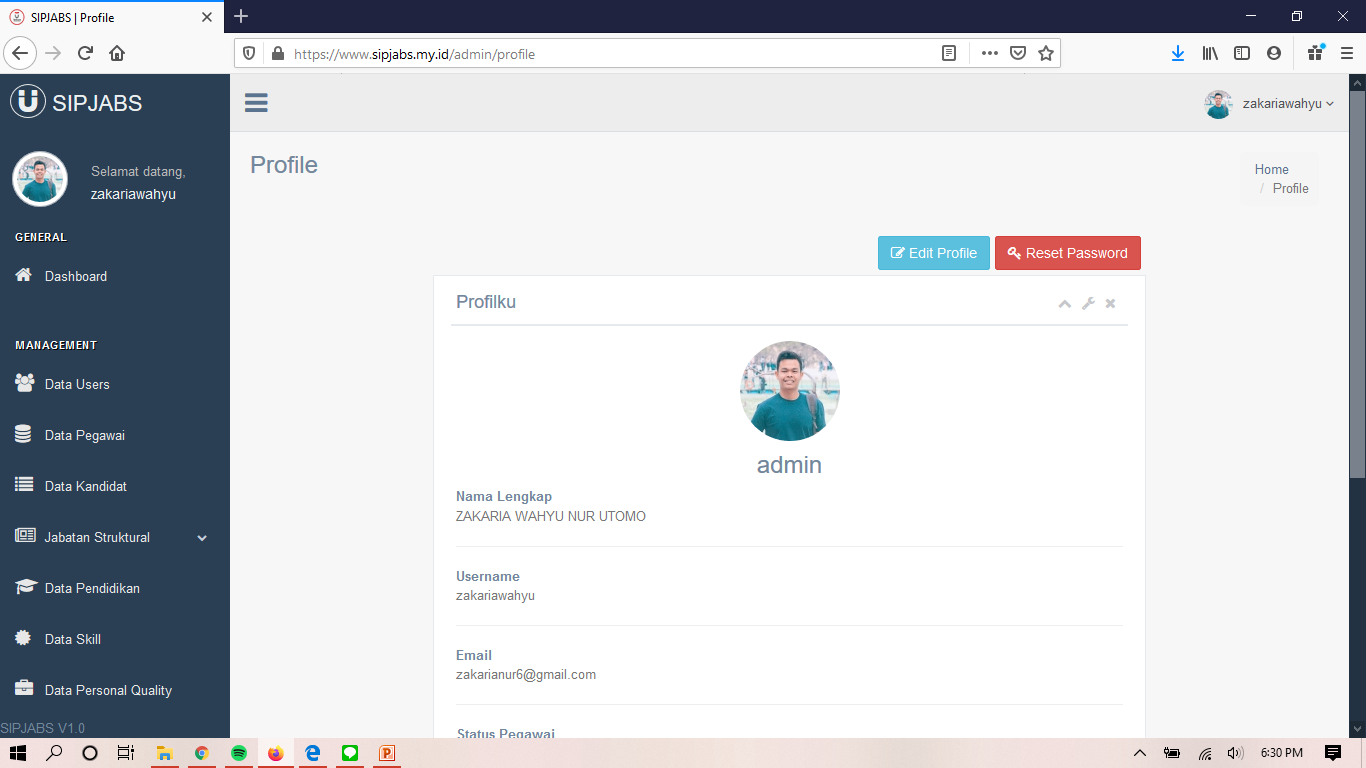
\includegraphics[width=0.8\textwidth]
		{pics/admin/implementasi/profile.png}
		\caption{Halaman \textit{Profile} Admin}
		\label{fig:CC10}
	\end{figure}
	Implementasi diatas menjelaskan bahwasannya admin dapat melihat \textit{profile} dengan mengklik \textit{username} yang berada di atas kanan, kemudian akan terdapat \textit{dropdown}, lalu klik \textit{profile}, maka akan tampil \textit{profile} dari admin.
	
	\item Halaman \textit{Edit Profile}
	\begin{figure}
		\centering
		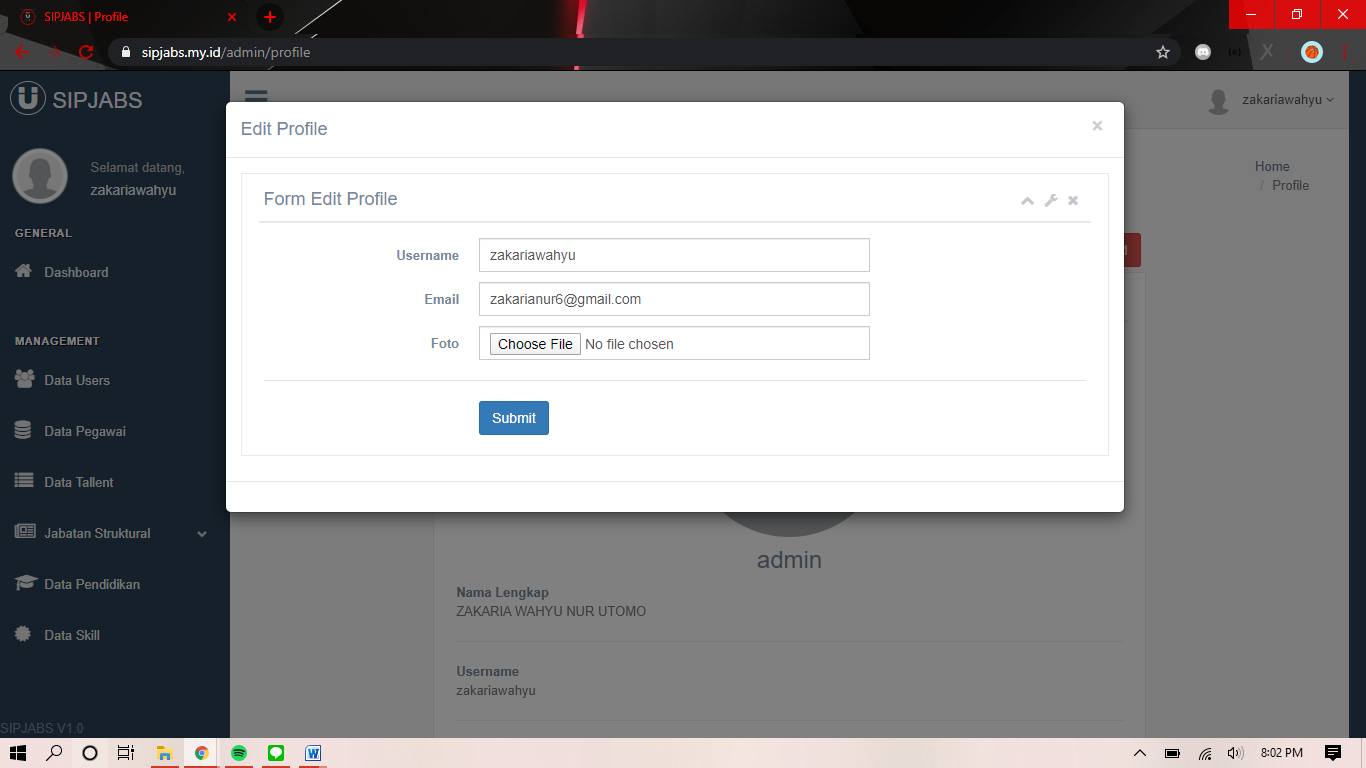
\includegraphics[width=0.8\textwidth]
		{pics/admin/implementasi/editprofile.png}
		\caption{Halaman \textit{Edit Profile} Admin}
		\label{fig:CC10}
	\end{figure}
	Gambar diatas mengimplementasikan bahwasannya admin dapat mengedit data \textit{profile} dengan mengklik \textit{button “edit profile”} kemudian dapat mengganti \textit{username} atau email dan foto. Lalu admin harus mengklik “\textit{submit}” untuk dapat menyimpan data yang sudah diperbarui. 
	
	\newpage
	\item Halaman \textit{Reset Password}
	\begin{figure}
		\centering
		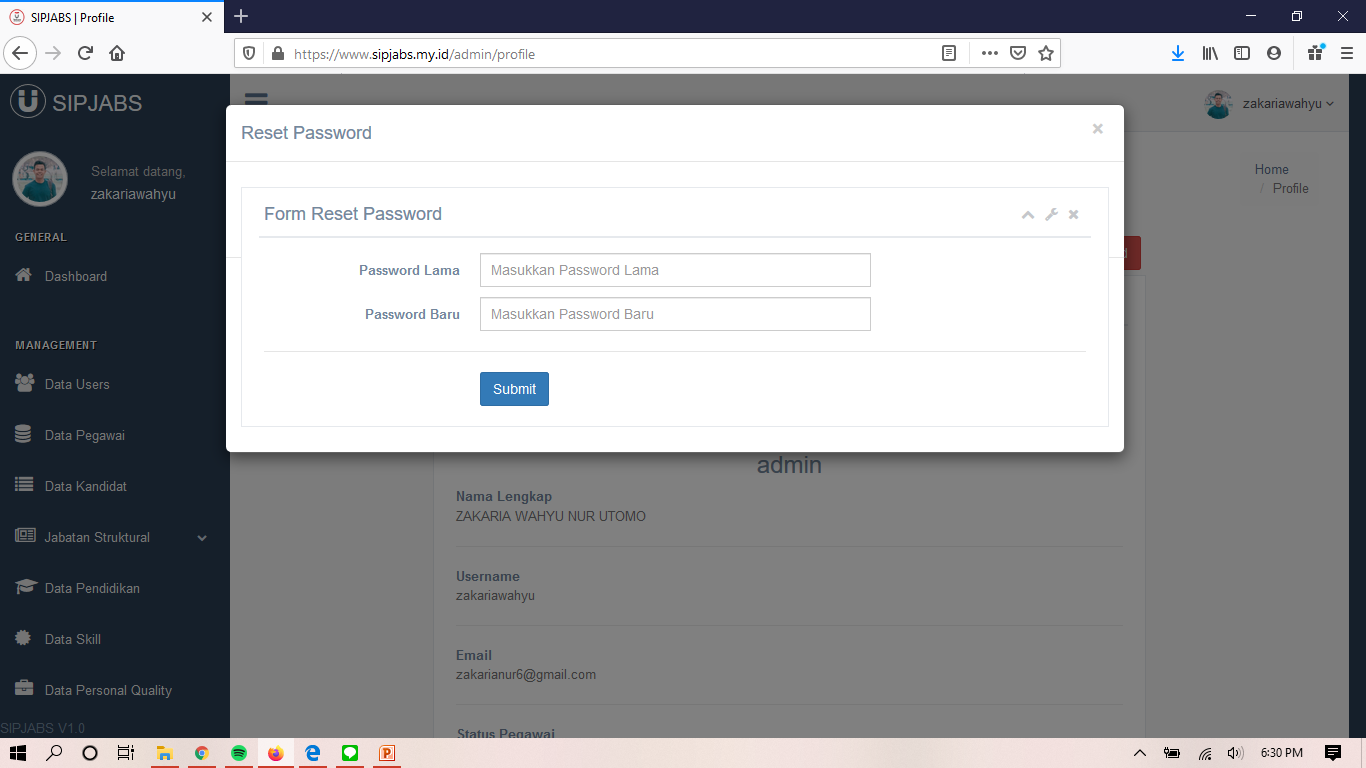
\includegraphics[width=0.8\textwidth]
		{pics/admin/implementasi/resetpassword.png}
		\caption{Halaman \textit{Reset Password} Admin}
		\label{fig:CC10}
	\end{figure}
	Implementasi diatas menandakan bahwasannya admin dapat mengganti \textit{password} apabila \textit{password} terebut sudah diketahui oleh pihak lain, dengan klik \textit{button “reset password”} kemudian akan tampil halaman \textit{pop-up} seperti diatas, admin cukup menginputkan \textit{password} lama dan \textit{password} baru, lalu klik “\textit{submit}” untuk menyimpan \textit{password} yang sudah diganti. 
	
	\item Halaman \textit{Help}
	\begin{figure}
		\centering
		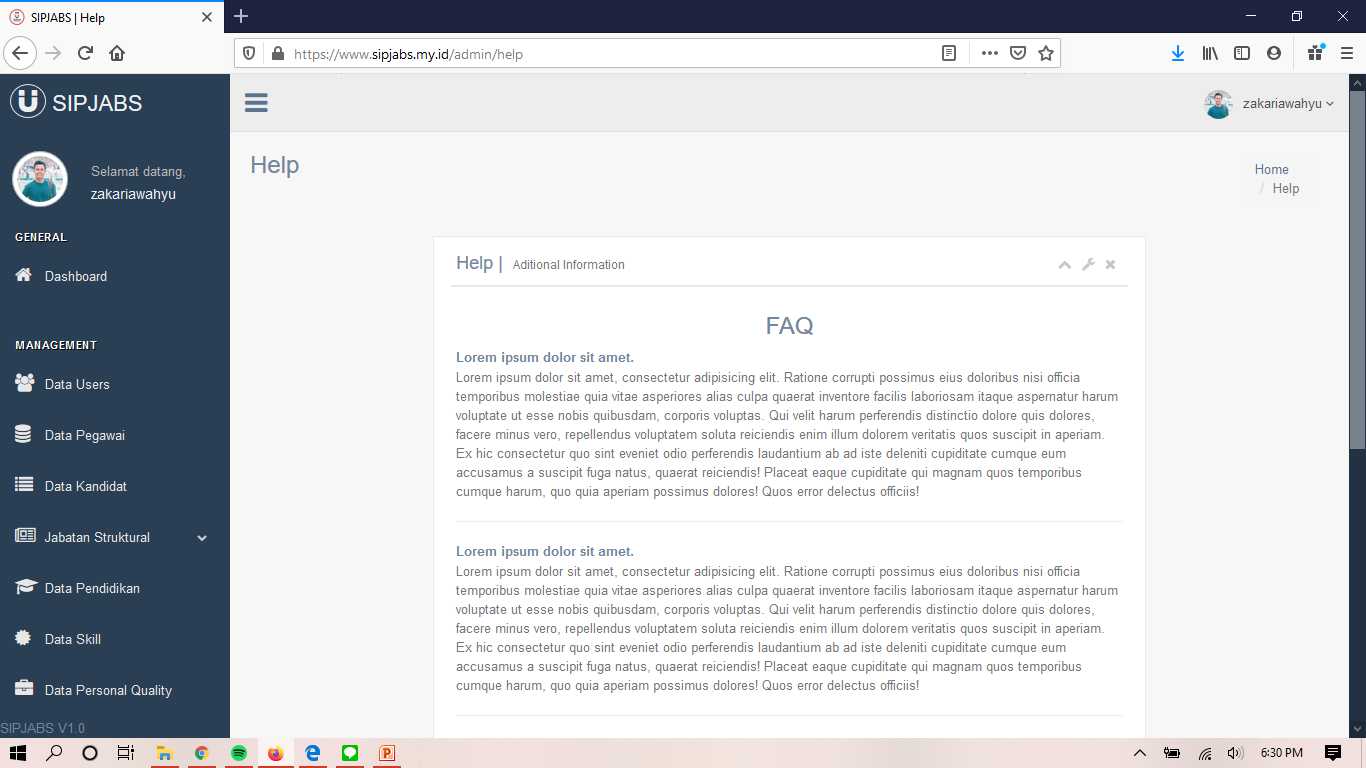
\includegraphics[width=0.8\textwidth]
		{pics/admin/implementasi/help.png}
		\caption{Halaman \textit{Help} Admin}
		\label{fig:CC10}
	\end{figure}

	\newpage
	\item Halaman Data \textit{Users}
	\begin{figure}
		\centering
		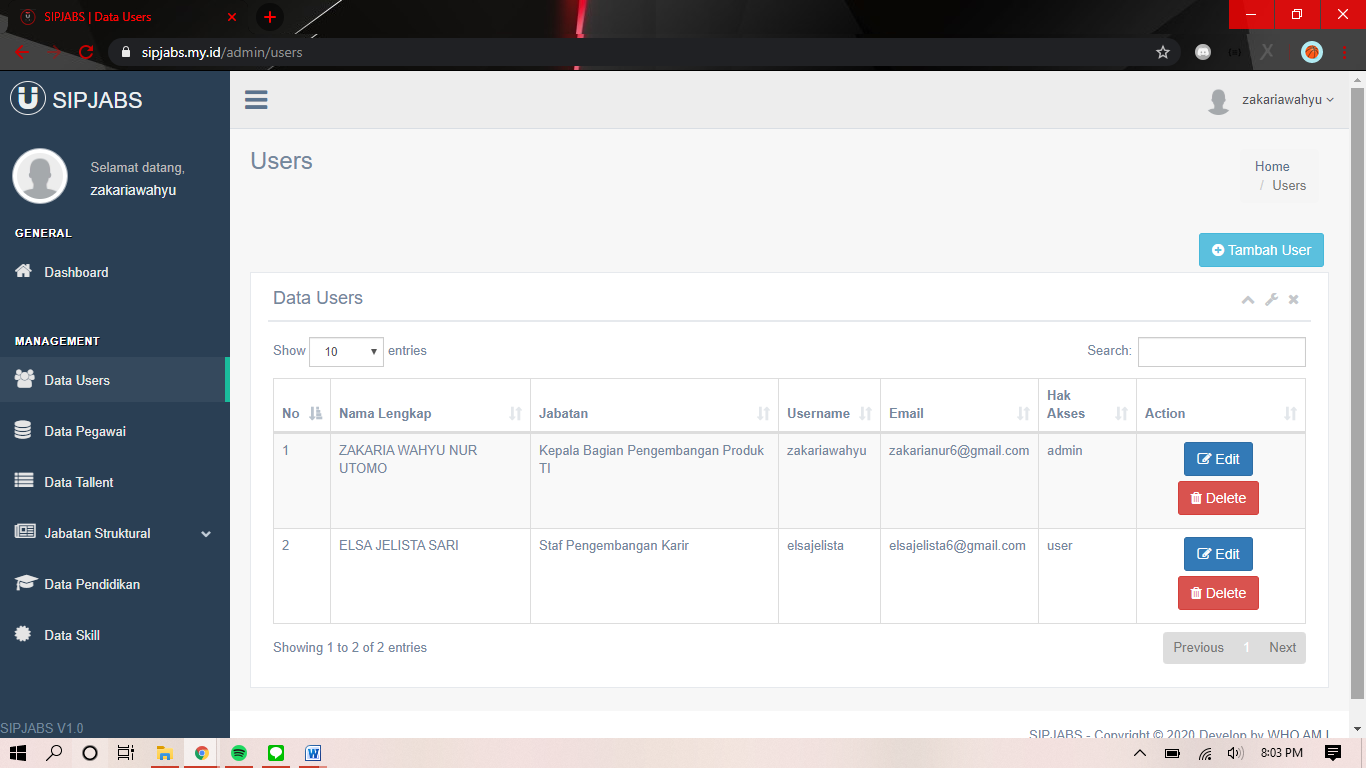
\includegraphics[width=0.8\textwidth]
		{pics/admin/implementasi/datausers.png}
		\caption{Halaman Data \textit{Users} - Admin}
		\label{fig:CC10}
	\end{figure}
	Gambar diatas menjelaskan isi dari halaman data \textit{users}, dimana admin dapat mengelola \textit{users} yang bisa mengakses aplikasi \textbf{SiPJabS}, karena apikasi ini hanya dapat diakses oleh orang-orang tententu. 
	
	\item Halaman \textit{Edit} Data \textit{Users}
	\begin{figure}
		\centering
		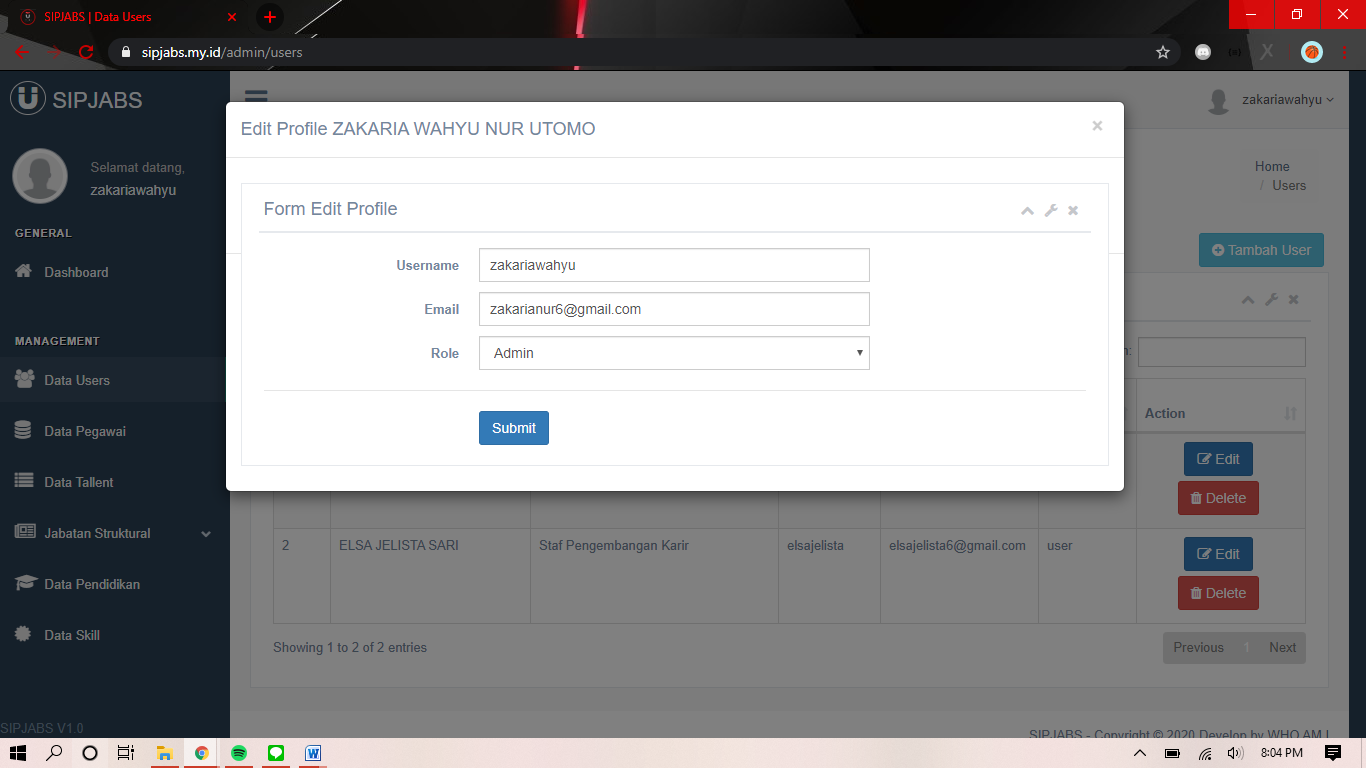
\includegraphics[width=0.8\textwidth]
		{pics/admin/implementasi/editusers.png}
		\caption{Halaman \textit{Edit} Data \textit{Users} - Admin}
		\label{fig:CC10}
	\end{figure}
	Gambar diatas menjelaskan bahwasannya data \textit{users} dapat diedit seperti \textit{username}, email, dan \textit{role} yang digunakan sebagai admin atau \textit{user}. Apabila data sudah diubah admin dapat mengklik \textit{button “Submit”} untuk menyelesaikan proses.
	
	\newpage
	\item Halaman Hapus \textit{Users}
	\begin{figure}
		\centering
		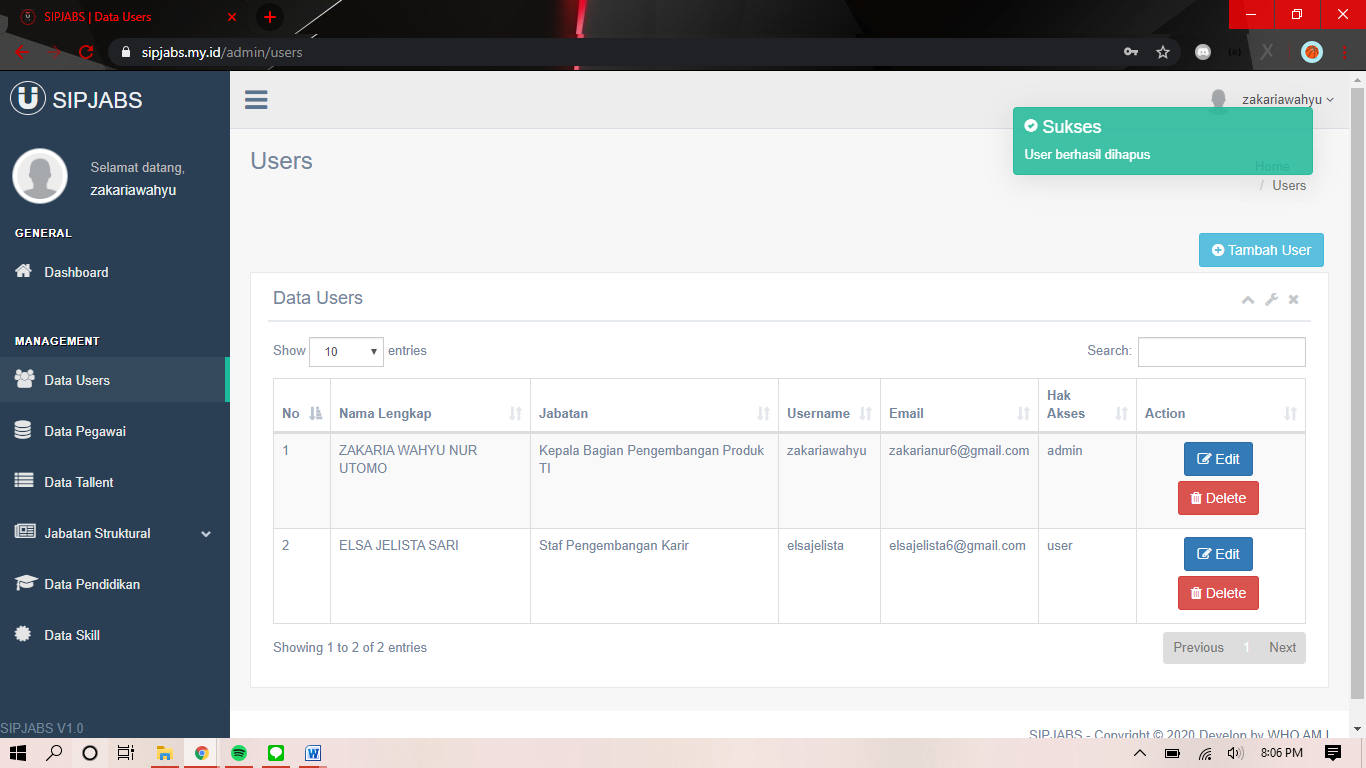
\includegraphics[width=0.8\textwidth]
		{pics/admin/implementasi/hapususers.png}
		\caption{Halaman Hapus \textit{Users} - Admin}
		\label{fig:CC10}
	\end{figure}
	Gambar diatas menjelaskan bahwasannya \textit{user} yang tidak bekerja lagi pada pengelolaan data tallent dapat dihapus dengan mengklik \textit{button delete}, kemudian akan terdapat \textit{pop-up} yang memiliki pesan “user berhasil dihapus”. 
	
	\item Halaman Tambah \textit{Users}
	\begin{figure}
		\centering
		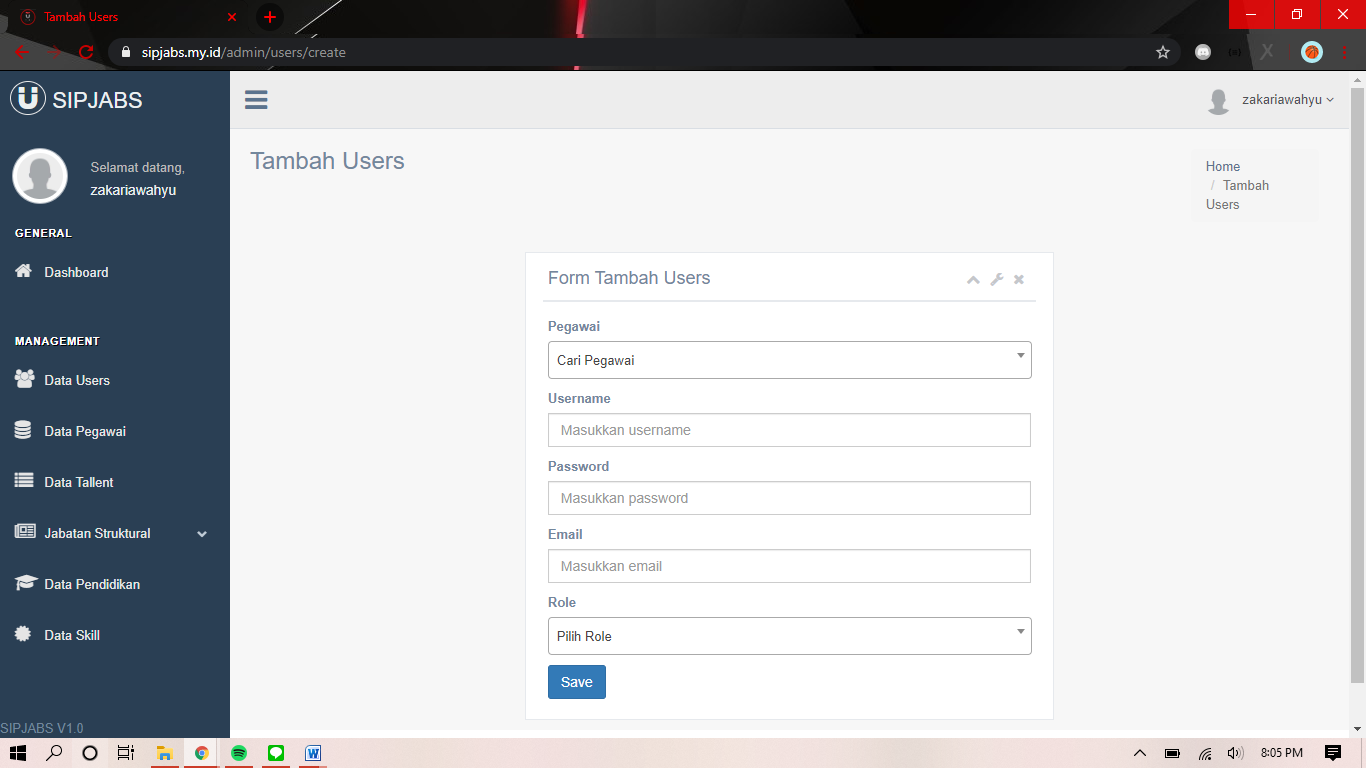
\includegraphics[width=0.8\textwidth]
		{pics/admin/implementasi/tambahusers.png}
		\caption{Halaman Tambah \textit{Users} - Admin}
		\label{fig:CC10}
	\end{figure}
	Dari tampilan diatas dapat dijelaskan, hanya admin saja yang dapat menambahkan data \textit{user}, namun harus sesuai dengan perintah dan \textit{job description} pegawai. Dengan mencari nama pegawai, menginputkan \textit{username}, \textit{password}, email, dan \textit{role}nya sebagai admin atau \textit{user}. Untuk mengakhiri proses admin dapat menyimpan apabila sudah disimpan akan terdapat \textit{pop-up}.
	
	\item Halaman Data Pegawai
	\begin{figure}
		\centering
		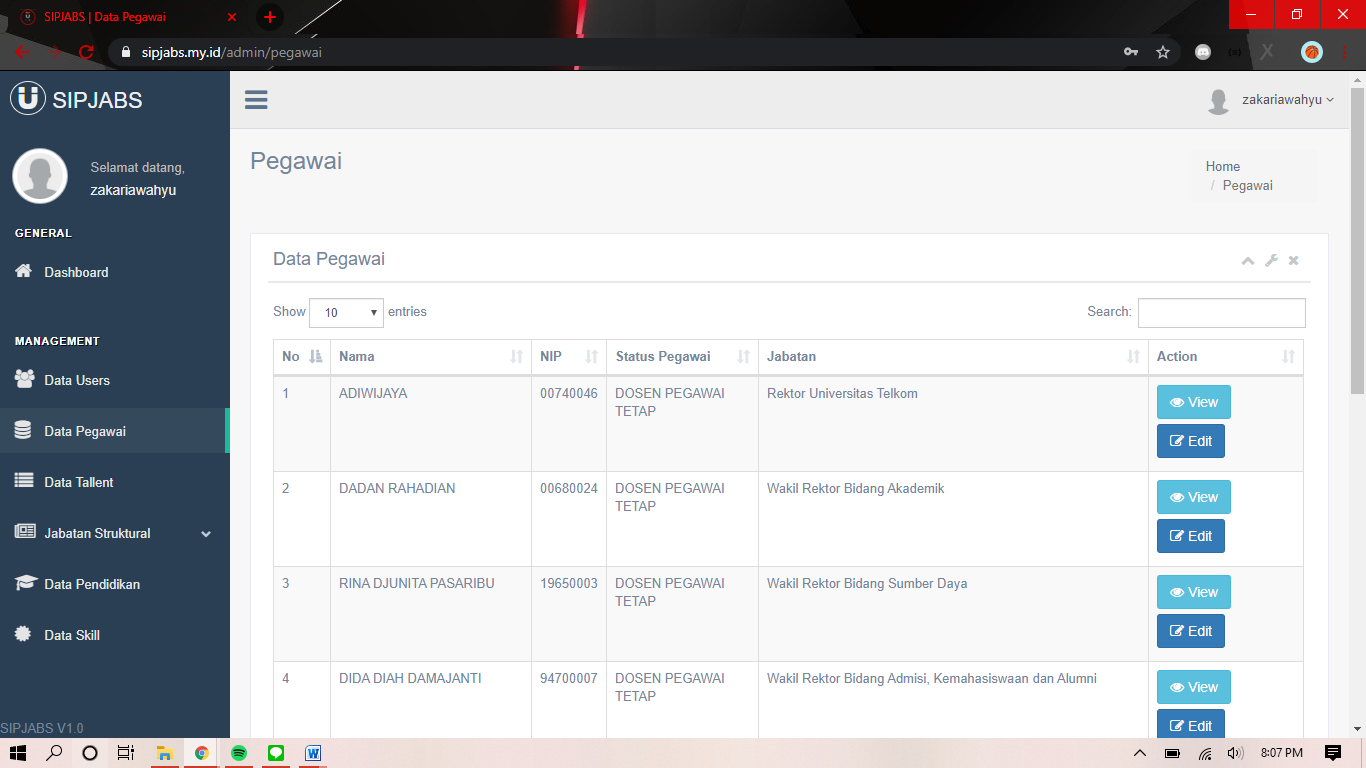
\includegraphics[width=0.8\textwidth]
		{pics/admin/implementasi/datapegawai.png}
		\caption{Halaman Data Pegawai - Admin}
		\label{fig:CC10}
	\end{figure}
	Dari tampilan diatas dijelaskan bahwasannya admin dapat melihat data seluruh pegawai yang ada di Universitas Telkom dengan mengklik menu “Data Pegawai” yang ada di sebelah kiri.
	
	\item Halaman \textit{View Detail} Pegawai
	\begin{figure}
		\centering
		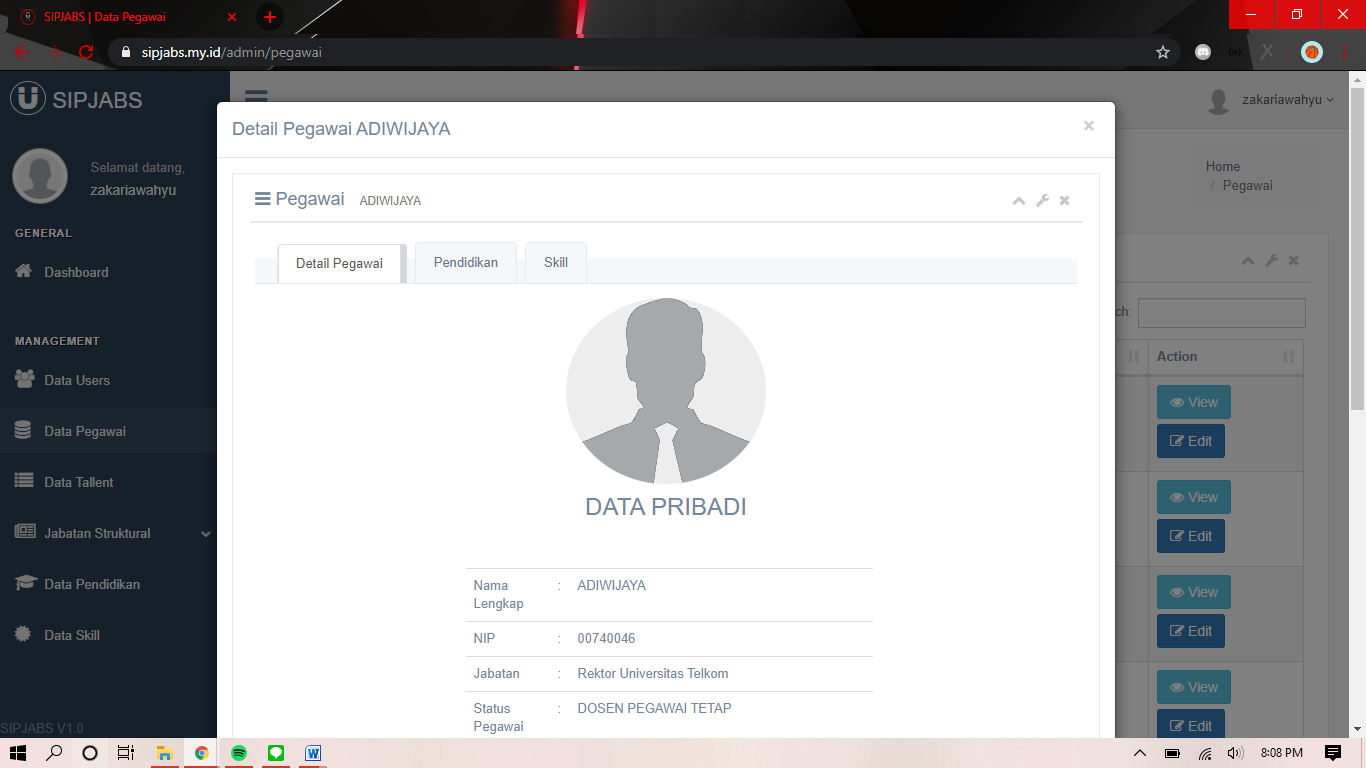
\includegraphics[width=0.8\textwidth]
		{pics/admin/implementasi/viewdetailpegawai.png}
		\caption{Halaman \textit{View Detail} Pegawai - Admin}
		\label{fig:CC10}
	\end{figure}
	Untuk implementasi \textit{view detail} pegawai admin dapat mengklik \textit{button view}, maka akan tampil seperti gambar diatas. Terdapat data pribadi dari pegawai yang dapat dilihat diantaranya: nama lengkap, NIP, jabatan, status pegawai, masa kerja, tempat lahir, tanggal lahir, status perkawinan, golongan darah, jenis kelamin, agama, tinggi badan, berat badan, dan alamat.
	
	\item Halaman Data \textit{Tallent}
	\begin{figure}
		\centering
		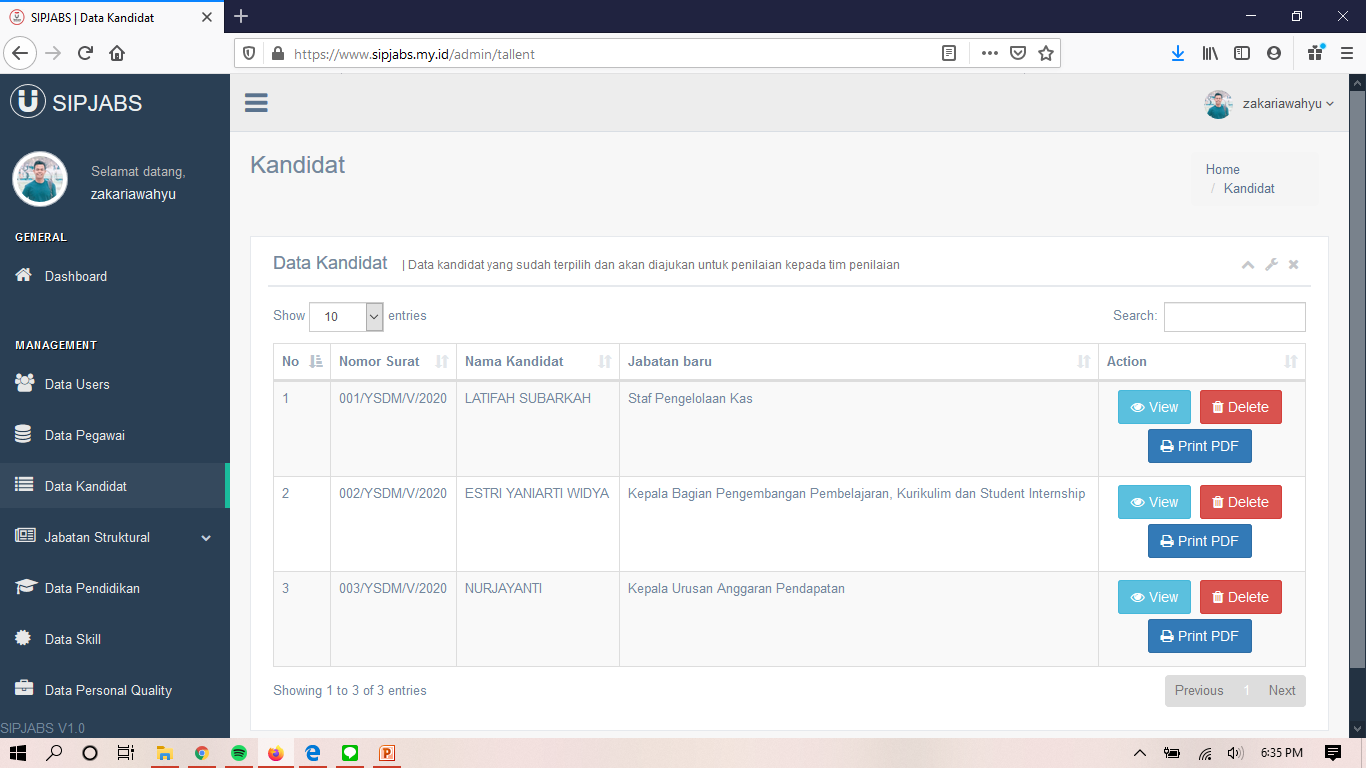
\includegraphics[width=0.8\textwidth]
		{pics/admin/implementasi/datatallent.png}
		\caption{Halaman Data \textit{Tallent} - Admin}
		\label{fig:CC10}
	\end{figure}
	Gambar diatas menampilkan halaman data \textit{tallent} yang dapat dilihat apabila admin mengklik menu “Data \textit{Tallent}”. Terdapat data tallent yang sudah dipilih oleh \textit{user}, sesuai dengan requitment yang telah ditetapkan perusahaan guna mengganti atau mengisi posisi yang kosong.  
	
	\item Halaman \textit{View Detail Tallent}
	\begin{figure}
		\centering
		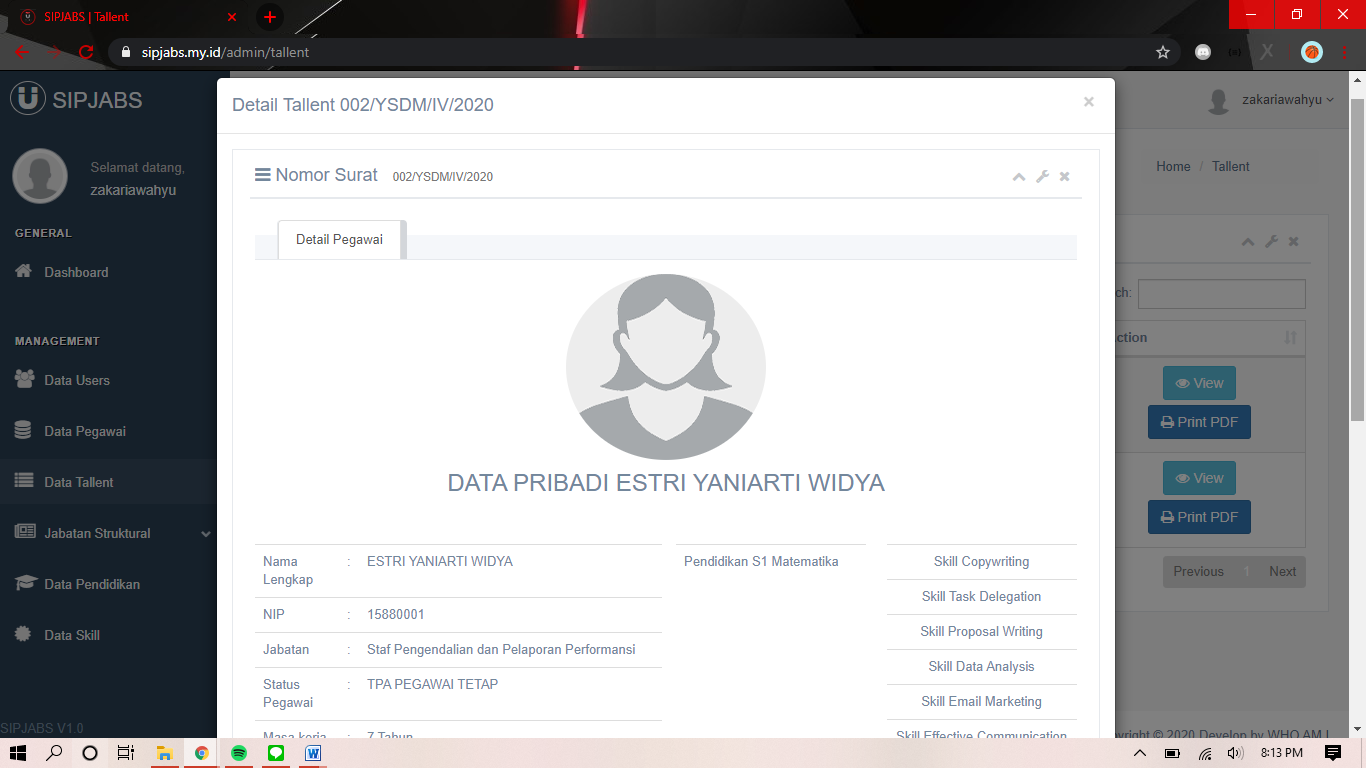
\includegraphics[width=0.8\textwidth]
		{pics/admin/implementasi/viewdetailtallent.png}
		\caption{Halaman \textit{View Detail Tallent} - Admin}
		\label{fig:CC10}
	\end{figure}
	Tampilan diatas akan muncul apabila admin mengklik \textit{button “view”}. Kemudian tampil \textit{detail} data pegawai yang suda dipilih oleh \textit{user}, seperti data pribadi, jenjang pendidikan, dan \textit{skill}. 
	
	\newpage
	\item Halaman Data Unit Kerja
	\begin{figure}
		\centering
		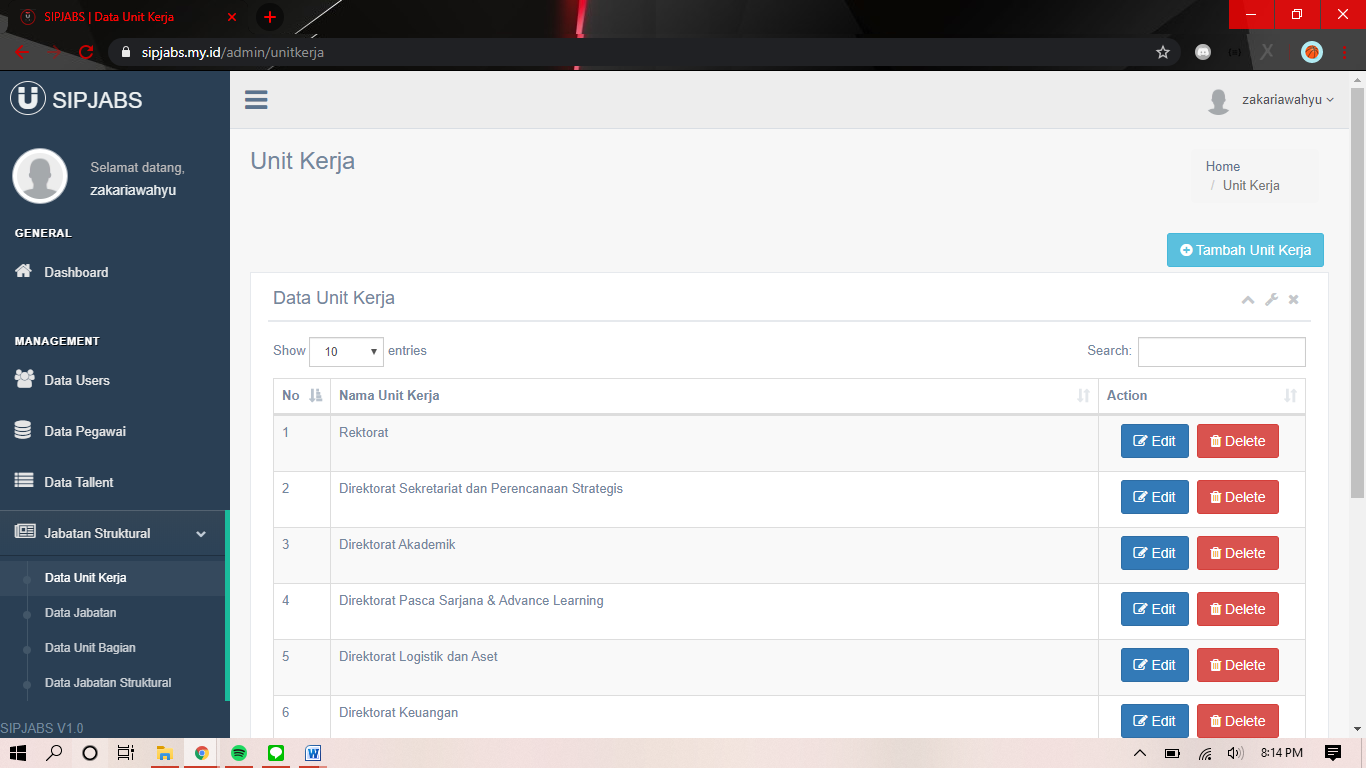
\includegraphics[width=0.8\textwidth]
		{pics/admin/implementasi/dataunitkerja.png}
		\caption{Halaman Data Unit Kerja - Admin}
		\label{fig:CC10}
	\end{figure}
	Untuk implementasi diatas admin harus klik “jabatan struktural” kemudian akan terdapat \textit{dropdown}, lalu klik “data unit kerja” maka akan menampilkan data unit kerja yang berada di Universitas Telkom dari rektorat hingga ke fakultas. 
	
	\item Halaman \textit{Edit} Unit Kerja
	\begin{figure}
		\centering
		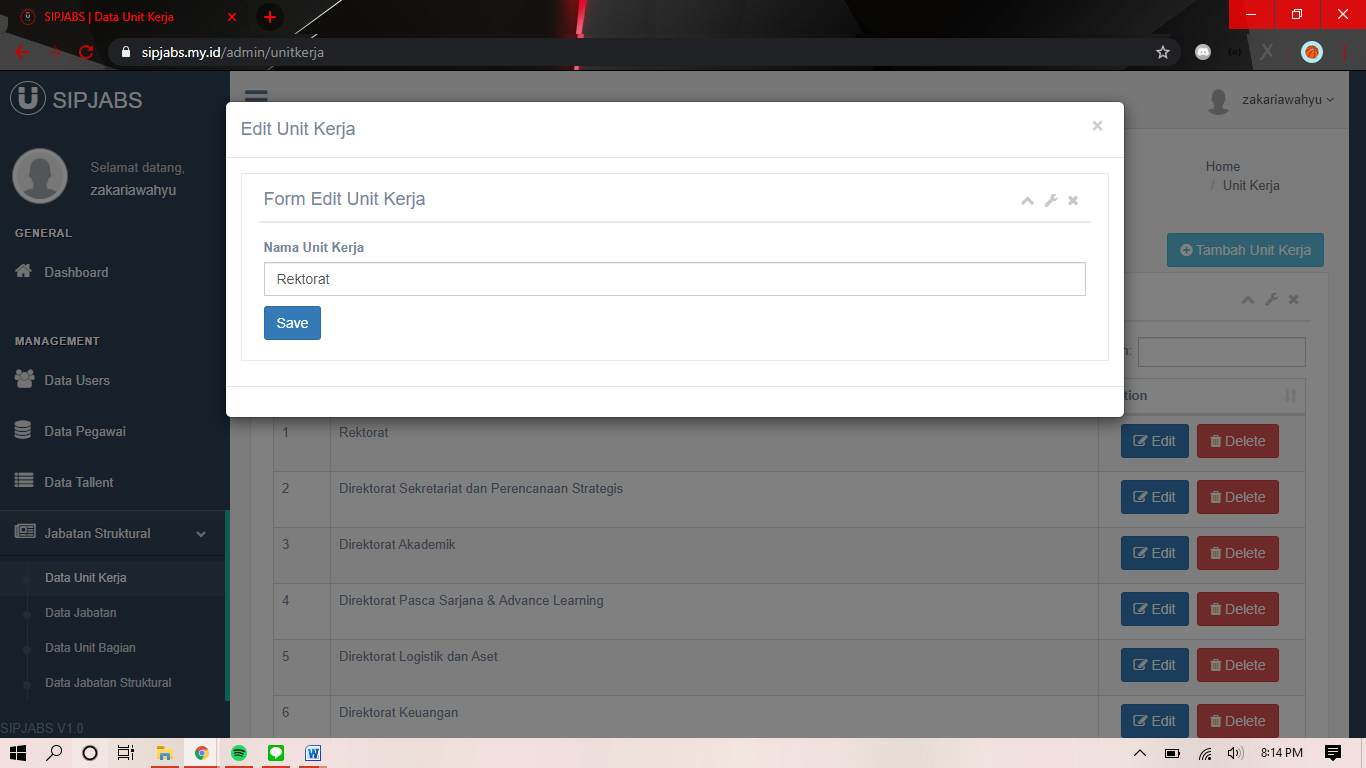
\includegraphics[width=0.8\textwidth]
		{pics/admin/implementasi/editunitkerja.png}
		\caption{Halaman \textit{Edit} Unit Kerja - Admin}
		\label{fig:CC10}
	\end{figure}
	Gambar diatas akan muncul apabila admin mengklik \textit{button “edit”} kemudian akan tampil \textit{pop-up} edit unit kerja, apabila nama unit kerja mengalami perubahan yang sudah ditetapkan. 
	
	\newpage
	\item Halaman Tambah Unit Kerja
	\begin{figure}
		\centering
		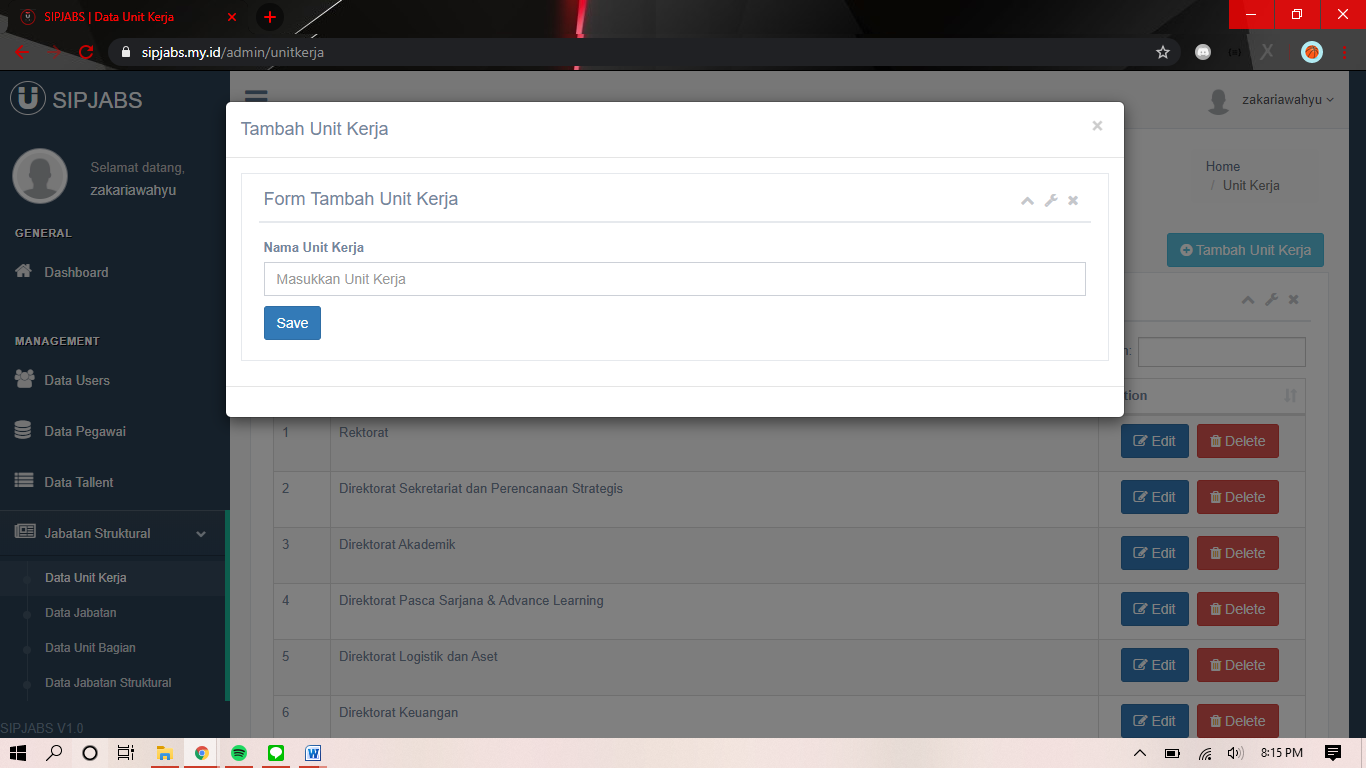
\includegraphics[width=0.8\textwidth]
		{pics/admin/implementasi/tambahunitkerja.png}
		\caption{Halaman Tambah Unit Kerja - Admin}
		\label{fig:CC10}
	\end{figure}
	Implementasi diatas akan muncul apabila admin mengklik \textit{button} “tambah unit kerja”, apabila terdapat unit kerja baru yang sudah ditetapkan, maka admin dapat menambahkannya. Untuk menyelesaikan proses admin harus mengklik \textit{button “save”}, kemudian data akan tersimpan.
	
	\item Halaman Data Jabatan
	\begin{figure}
		\centering
		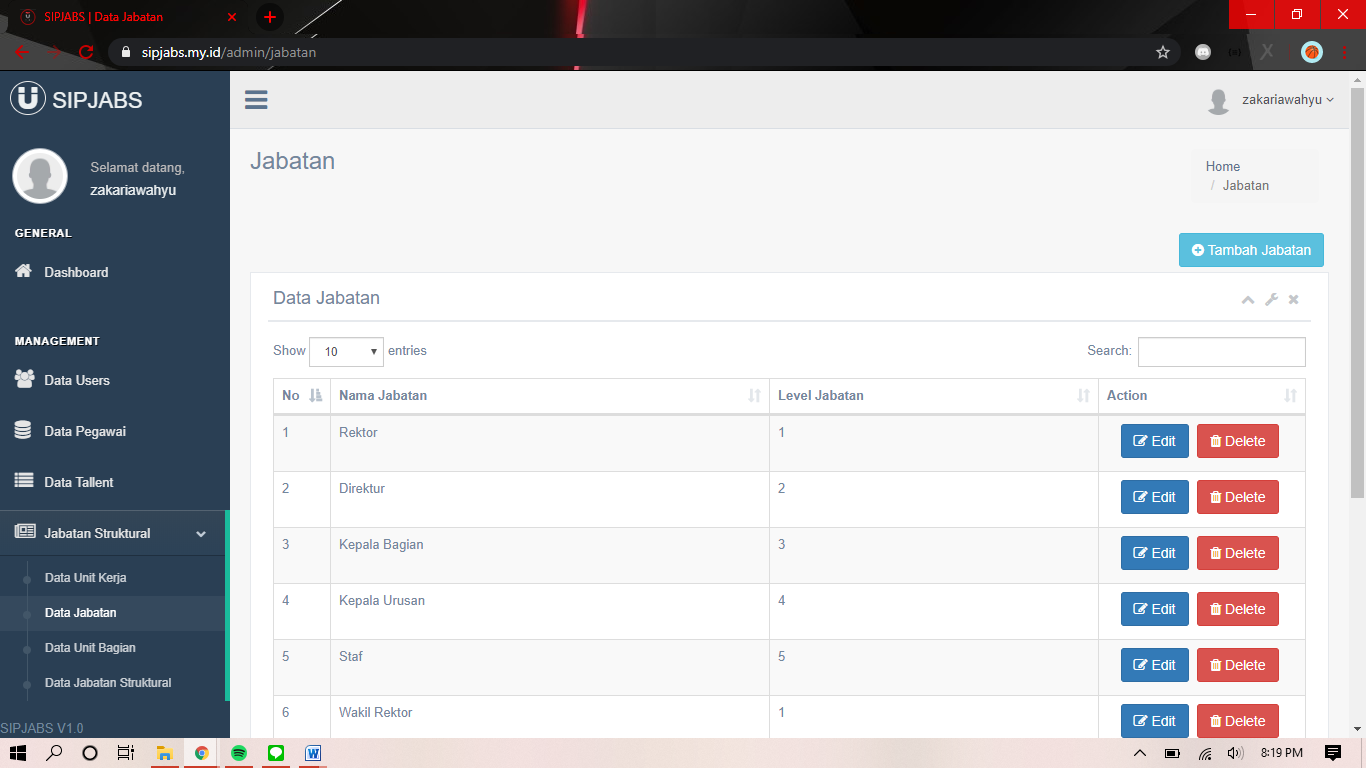
\includegraphics[width=0.8\textwidth]
		{pics/admin/implementasi/datajabatan.png}
		\caption{Halaman Data Jabatan - Admin}
		\label{fig:CC10}
	\end{figure}
	Gambar diatas menampilkan data jabatan apabila admin mengklik menu “data jabatan” pada \textit{dropdown} ”jabatan struktural”. Terdapat nama-nama jabatan yang ada di Universitas Telkom yang akan terhubung dengan unit kerja dan unit bagian.  
	
	\item Halaman \textit{Edit} Jabatan
	\begin{figure}
		\centering
		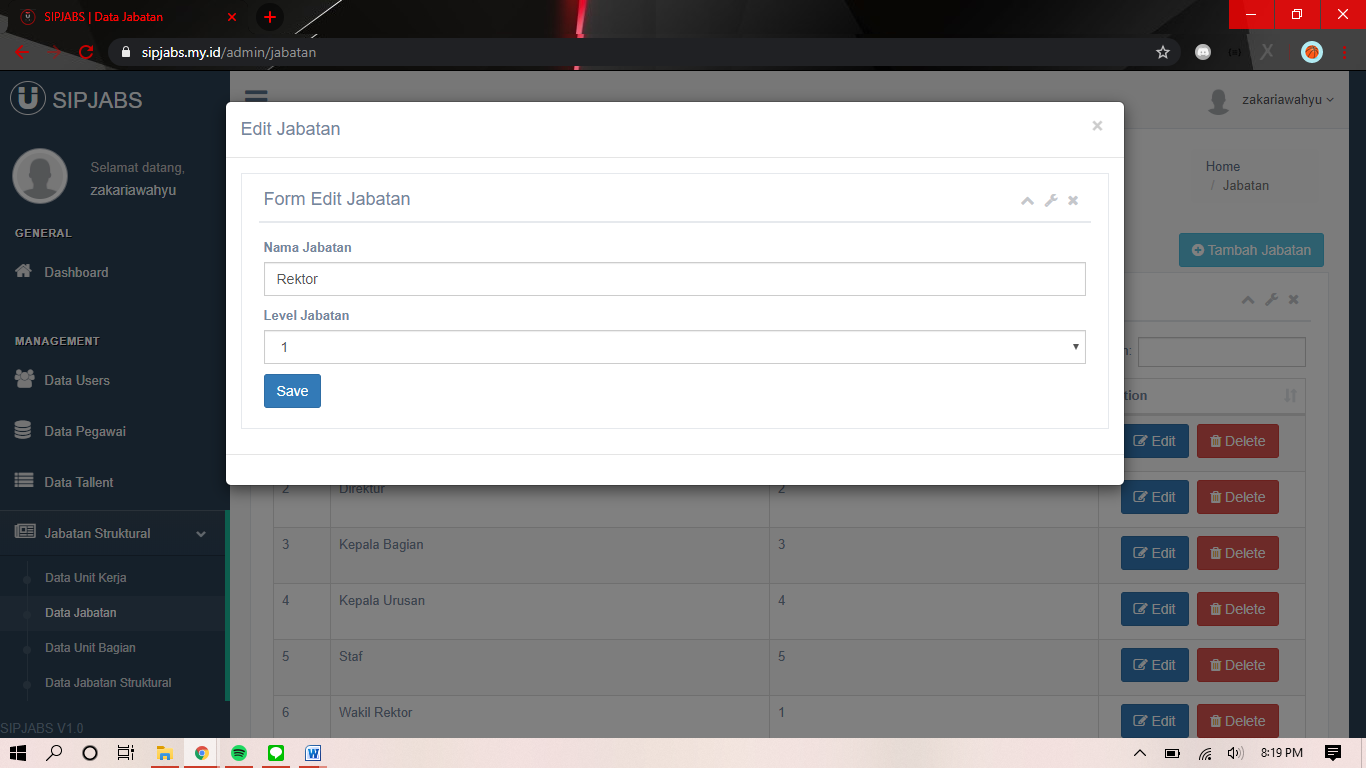
\includegraphics[width=0.8\textwidth]
		{pics/admin/implementasi/editjabatan.png}
		\caption{Halaman \textit{Edit} Jabatan - Admin}
		\label{fig:CC10}
	\end{figure}
	Untuk tampilan diatas adalah \textit{form edit} jabatan, admin dapat mengklik \textit{button “edit”} kemudian menginputkan nama jabatan serta level jabatan, dan menyimpannya untuk mengakhiri proses, kemudian data akan tersimpan.
	
	\item Halaman Tambah Jabatan
	\begin{figure}
		\centering
		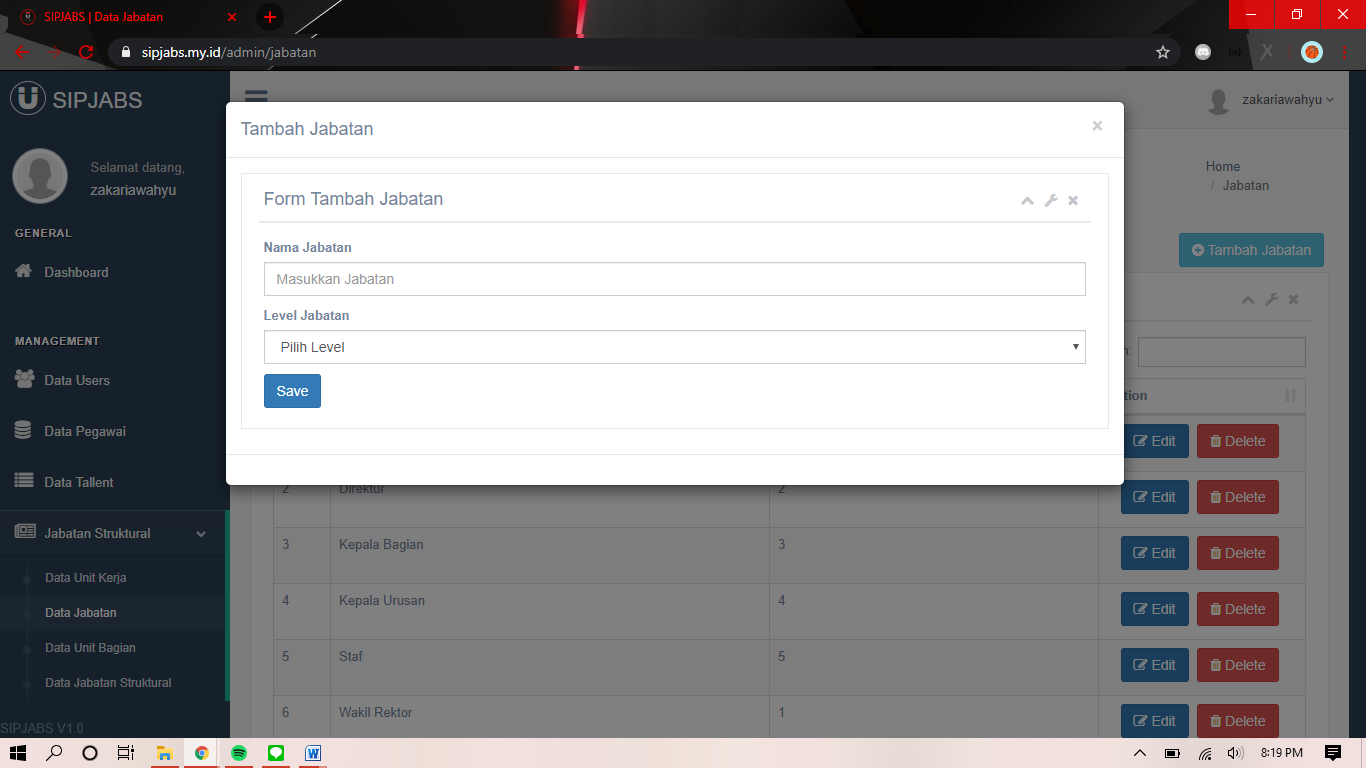
\includegraphics[width=0.8\textwidth]
		{pics/admin/implementasi/tambahjabatan.png}
		\caption{Halaman Tambah Jabatan - Admin}
		\label{fig:CC10}
	\end{figure}
	Gambar diatas menampilkan \textit{pop-up form} tambah jabatan, tampilan tersebut akan muncul apabila admin mengklik \textit{button} “tambah jabatan”. Kemudian admin menginputkan nama jabatan dan level jabatan untuk membuat jabatan baru yang sudah ditetapkan. Lalu simpan data tersebut dengan mengklik \textit{button “save”} maka data akan tesimpan di jabatan.
	
	\item Halaman Data Unit Bagian
	\begin{figure}
		\centering
		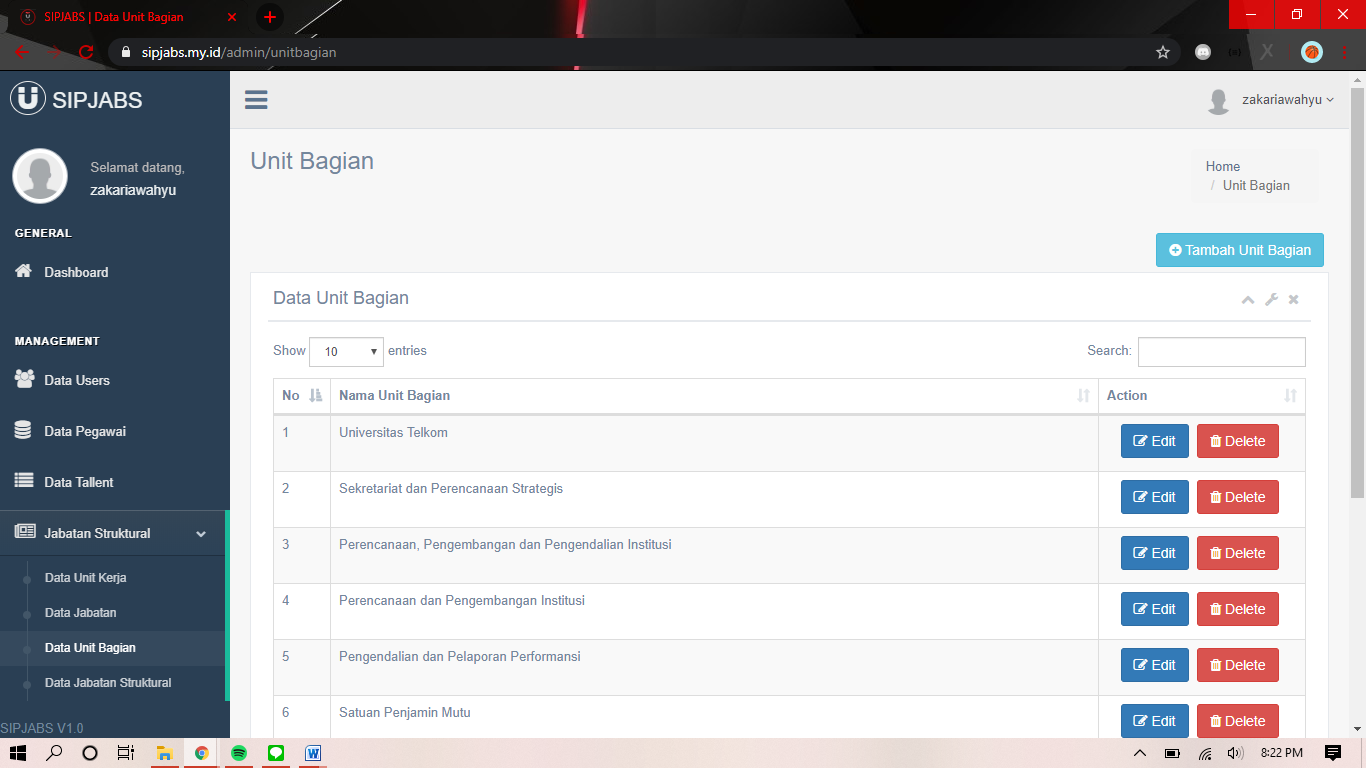
\includegraphics[width=0.8\textwidth]
		{pics/admin/implementasi/dataunitbagian.png}
		\caption{Halaman Data Unit Bagian - Admin}
		\label{fig:CC10}
	\end{figure}
	Untuk tampilan diatas adalah tampilan dari data unit bagian, didapat apabila admin mengklik \textit{dropdown} “jabatan struktural” pada menu kemudian mengklik “data unit bagian”, halaman ini menjelaskan bagian dari unit kerja yang ada di Universitas Telkom. Diharapkan dapat menyelesaikan pekerjaan sesuai dengan unit bagian masing-masing secara efektif dan maksimal.
	
	\item Halaman \textit{Edit} Unit Bagian
	\begin{figure}
		\centering
		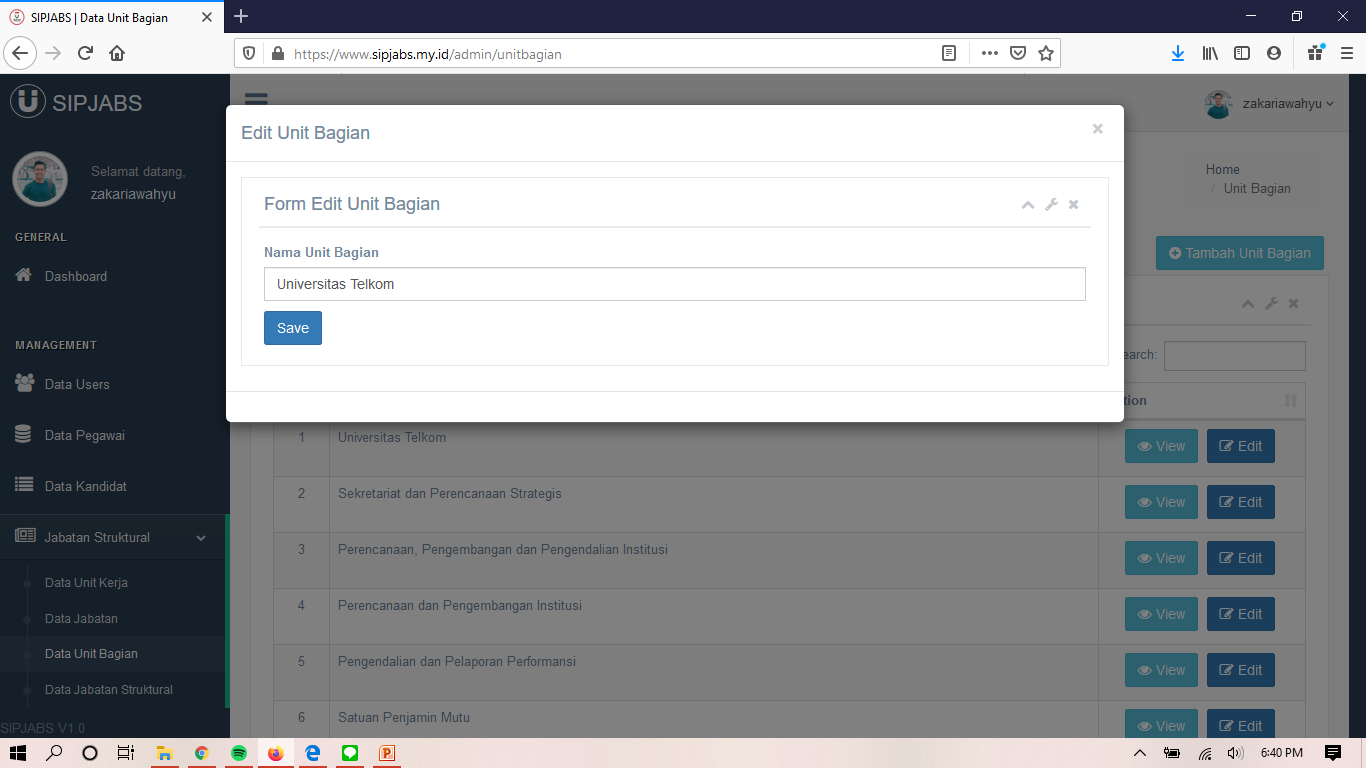
\includegraphics[width=0.8\textwidth]
		{pics/admin/implementasi/editunitbagian.png}
		\caption{Halaman \textit{Edit} Unit Bagian - Admin}
		\label{fig:CC10}
	\end{figure}
	Gambar diatas menampilkan \textit{form edit} unit bagian, didapat apabila admin mengklik \textit{button ”edit”} kemudian admin dapat menginputkan nama unit bagian yang baru dan sesuai dengan ketetapan, terakhir klik \textit{button “save”} sehingga data akan tersimpan kembali.
	
	\item Halaman Tambah Unit Bagian
	\begin{figure}
		\centering
		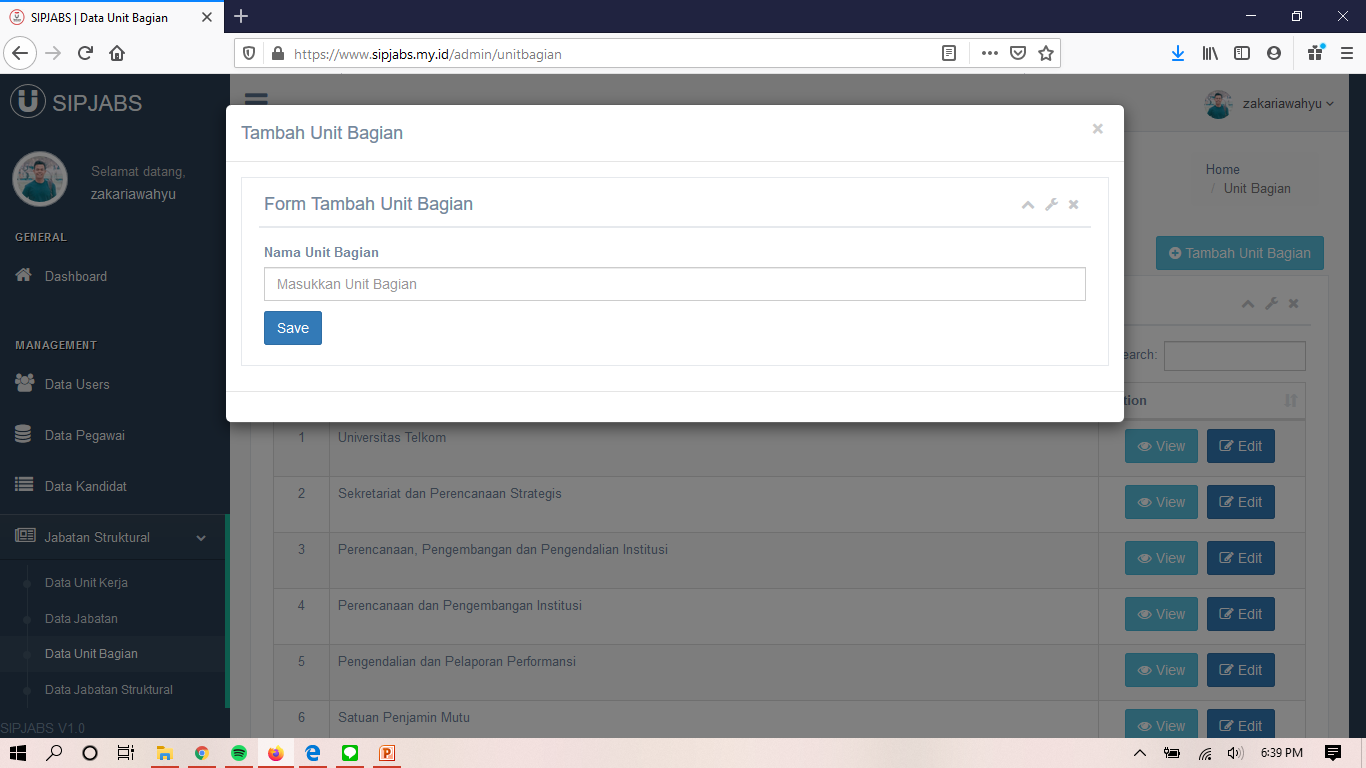
\includegraphics[width=0.8\textwidth]
		{pics/admin/implementasi/tambahunitbagian.png}
		\caption{Halaman Tambah Unit Bagian - Admin}
		\label{fig:CC10}
	\end{figure}
	Implementasi diatas menunjukkan bahwasannya admin dapat menambah data unit bagian dengan cara klik \textit{button} “tambah unit bagian” dan menginputkan nama unit bagian dan menyimpannya dengan mengklik \textit{button “save”}, kemudian data akan tersimpan didalam data unit bagian. 
	
	\item Halaman Data Jabatan Struktural
	\begin{figure}
		\centering
		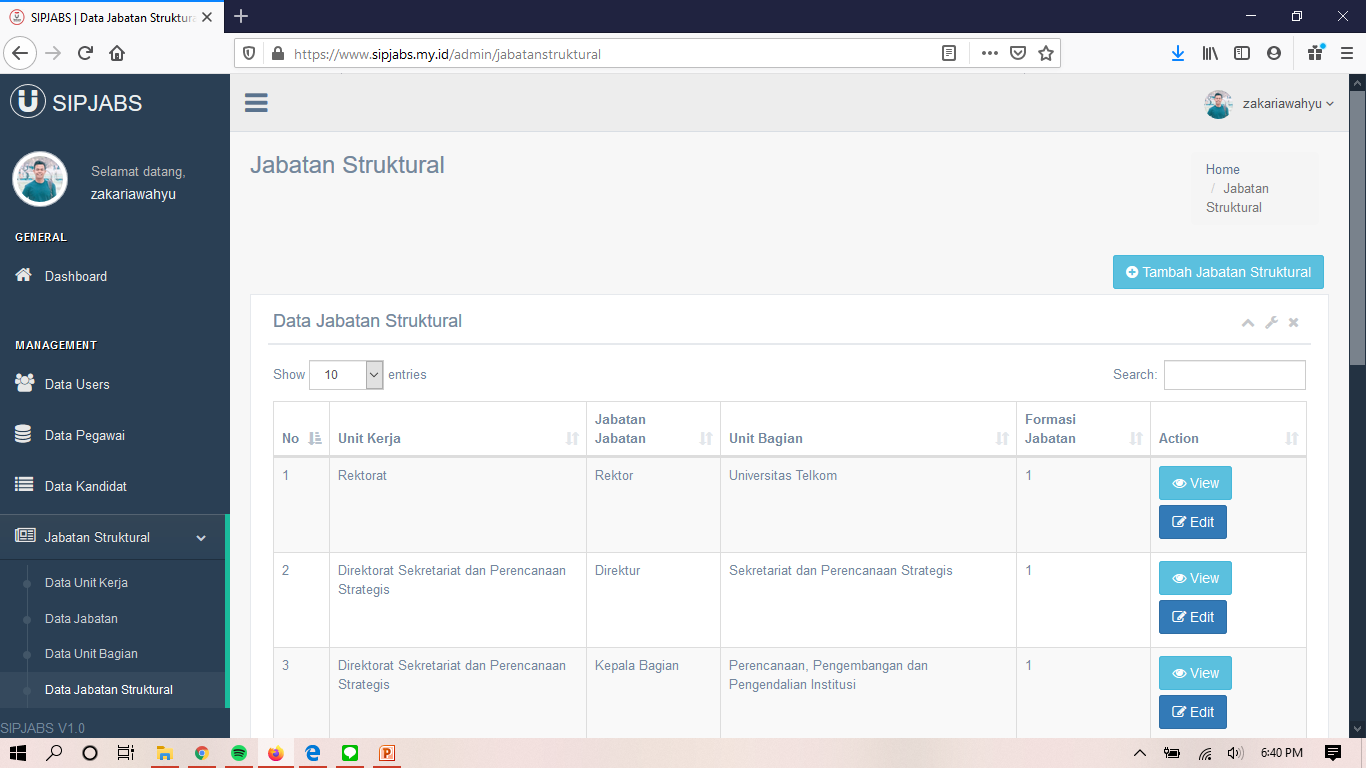
\includegraphics[width=0.8\textwidth]
		{pics/admin/implementasi/datajabstruk.png}
		\caption{Halaman Data Jabatan Struktural - Admin}
		\label{fig:CC10}
	\end{figure}
	Untuk implementasi dari tampilan diatas admin dapat mengklik \textit{dropdown} “jabatan struktural” kemudian mengklik menu “data jabatan struktural”, makan akan tampil halaman jabatan struktural yang ada di Universitas Telkom. Terdiri dari unit kerja, jabatan, unit bagian serta formasi jabatan. 
	
	\item Halaman \textit{Edit} Jabatan Struktural
	\begin{figure}
		\centering
		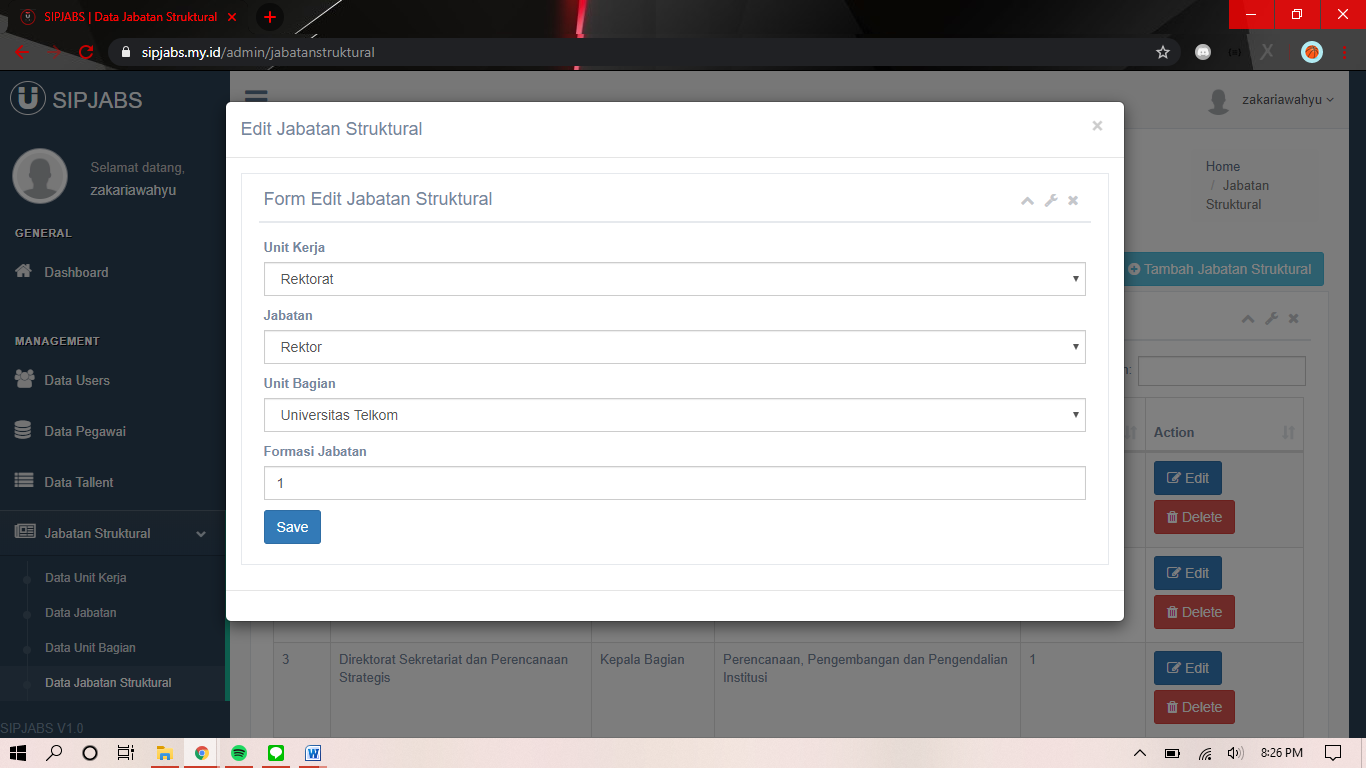
\includegraphics[width=0.8\textwidth]
		{pics/admin/implementasi/editjabstruk.png}
		\caption{Halaman \textit{Edit} Jabatan Struktural - Admin}
		\label{fig:CC10}
	\end{figure}
	Gambar diatas mengimplementasikan \textit{pop-up} dari \textit{form edit} jabatan struktural, dimana admin harus menginputkan unit kerja, jabatan, unit bagian, dan formasi jabatan, lalu untuk mengakhiri proses admin harus mengklik \textit{button “save”} kemudian data yang diedit akan tersimpan. 
	
	\item Halaman Tambah Jabatan Struktural
	\begin{figure}
		\centering
		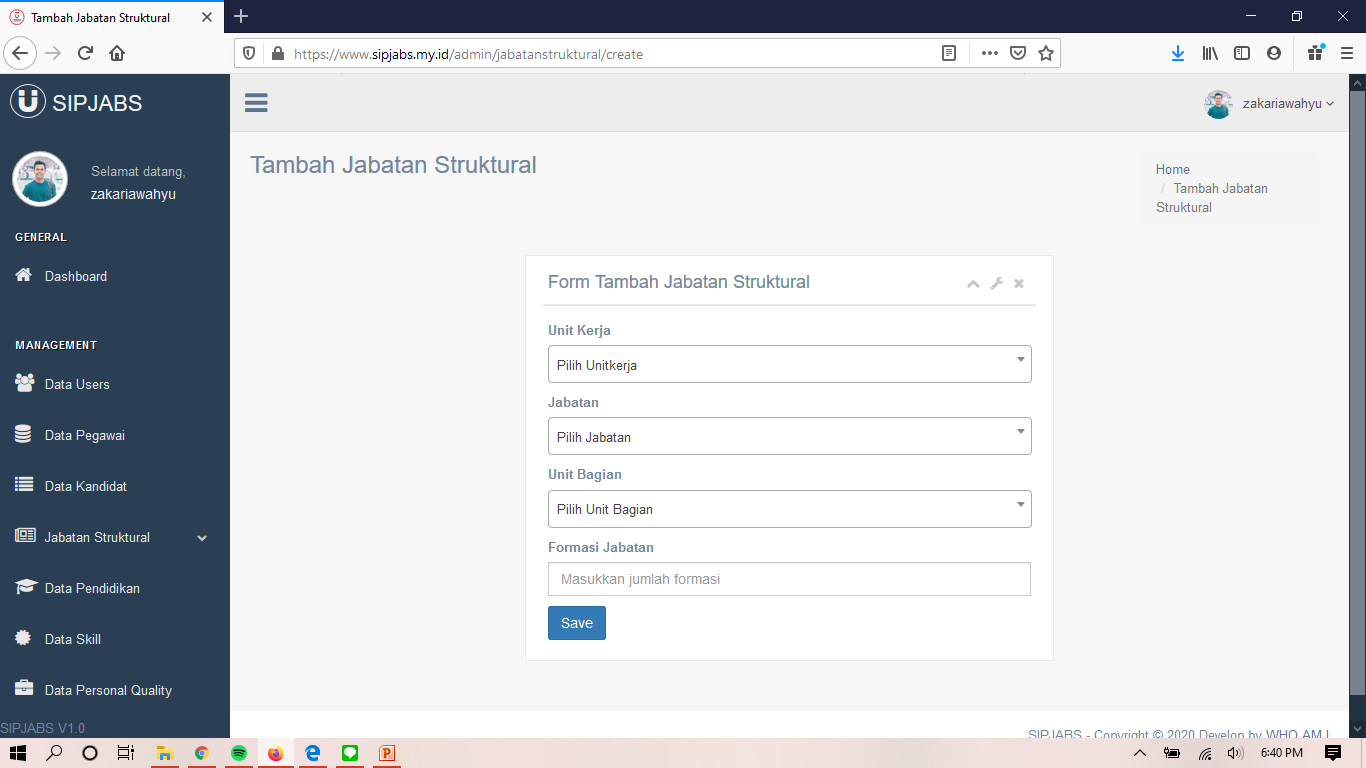
\includegraphics[width=0.8\textwidth]
		{pics/admin/implementasi/tambahjabstruk.png}
		\caption{Halaman Tambah Jabatan Struktural - Admin}
		\label{fig:CC10}
	\end{figure}
	Untuk tampilan diatas adalah \textit{form} tambah jabatan stuktural, didapat apabila admin mengklik \textit{button} “tambah jabatan struktural”, kemudian admin harus menginputkan data seperti unit kerja, jabatan, unit bagian, dan formasi jabatan, kemudian klik \textit{button “save”} untuk mengakhiri proses.
	
	\item Halaman Data Pendidikan
	\begin{figure}
		\centering
		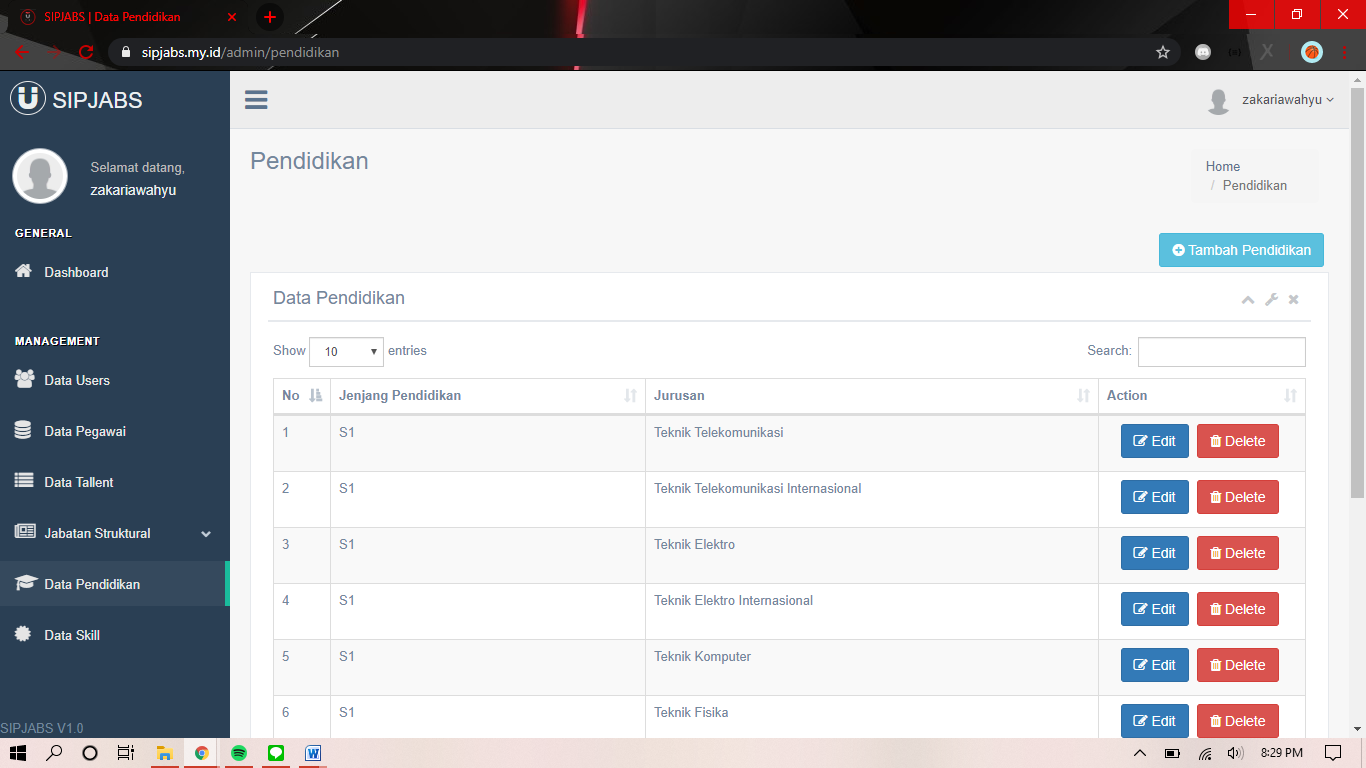
\includegraphics[width=0.8\textwidth]
		{pics/admin/implementasi/datapendidikan.png}
		\caption{Halaman Data Pendidikan - Admin}
		\label{fig:CC10}
	\end{figure}
	Gambar diatas menjelaskan data pendidikan semua pegawai Universitas Tekom, sehingga admin dapat mengetahui bahwasannya pegawai di Universitas Telkom memiliki jenjang pendidikan dan jurusan apa saja. Didapat apabila admin megklik menu “data pendidikan”.
	
	\item Halaman \textit{Edit} Pendidikan
	\begin{figure}
		\centering
		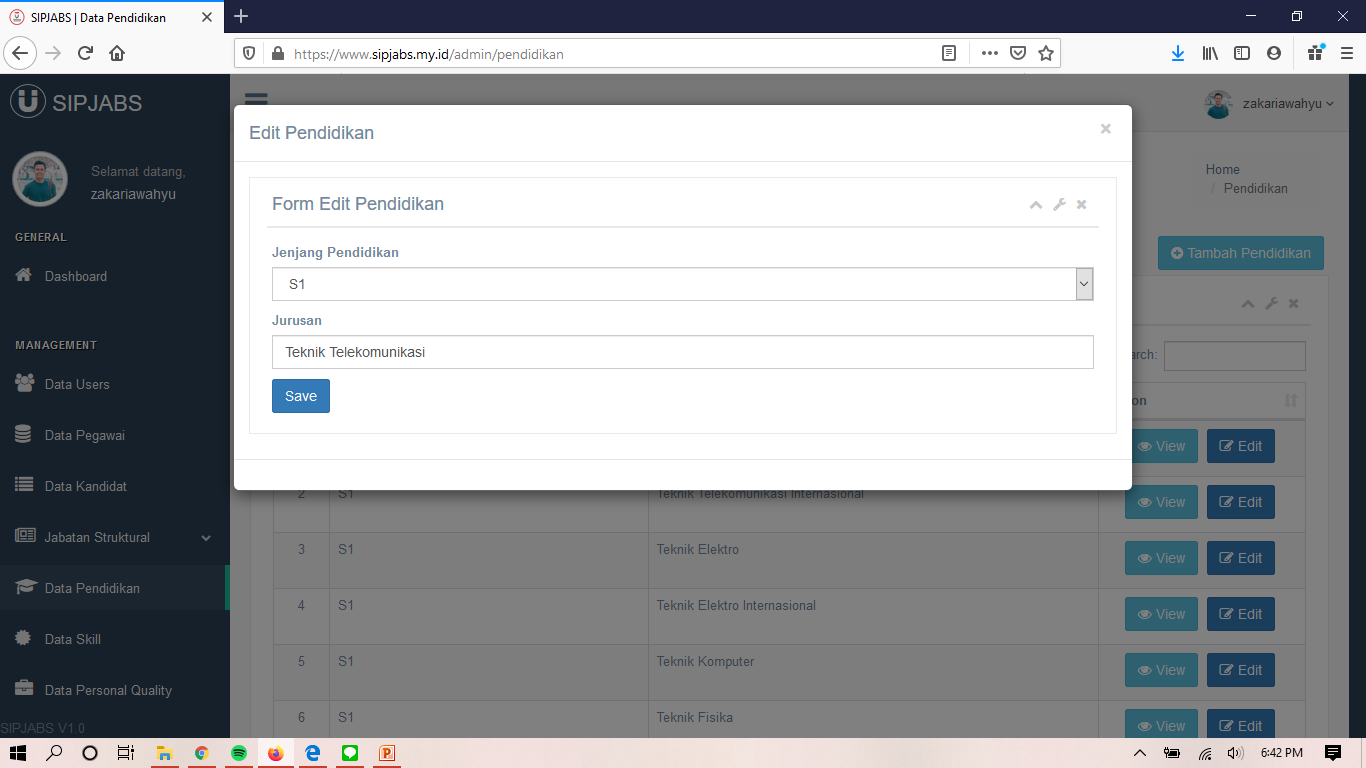
\includegraphics[width=0.8\textwidth]
		{pics/admin/implementasi/editpendidikan.png}
		\caption{Halaman \textit{Edit} Pendidikan - Admin}
		\label{fig:CC10}
	\end{figure}
	Untuk tampilan diatas adalah tampilan \textit{pop-up} dari \textit{form edit} pendidikan, apabila admin ingin mengedit data pendidikan dengan mengklik \textit{button “edit”} kemudian memilih jenjang pendidikan dan menginputkan jurusan, apabila sudah sesuai klik \textit{button “save”} untuk menyimpan data.
	
	\item Halaman Tambah Pendidikan
	\begin{figure}
		\centering
		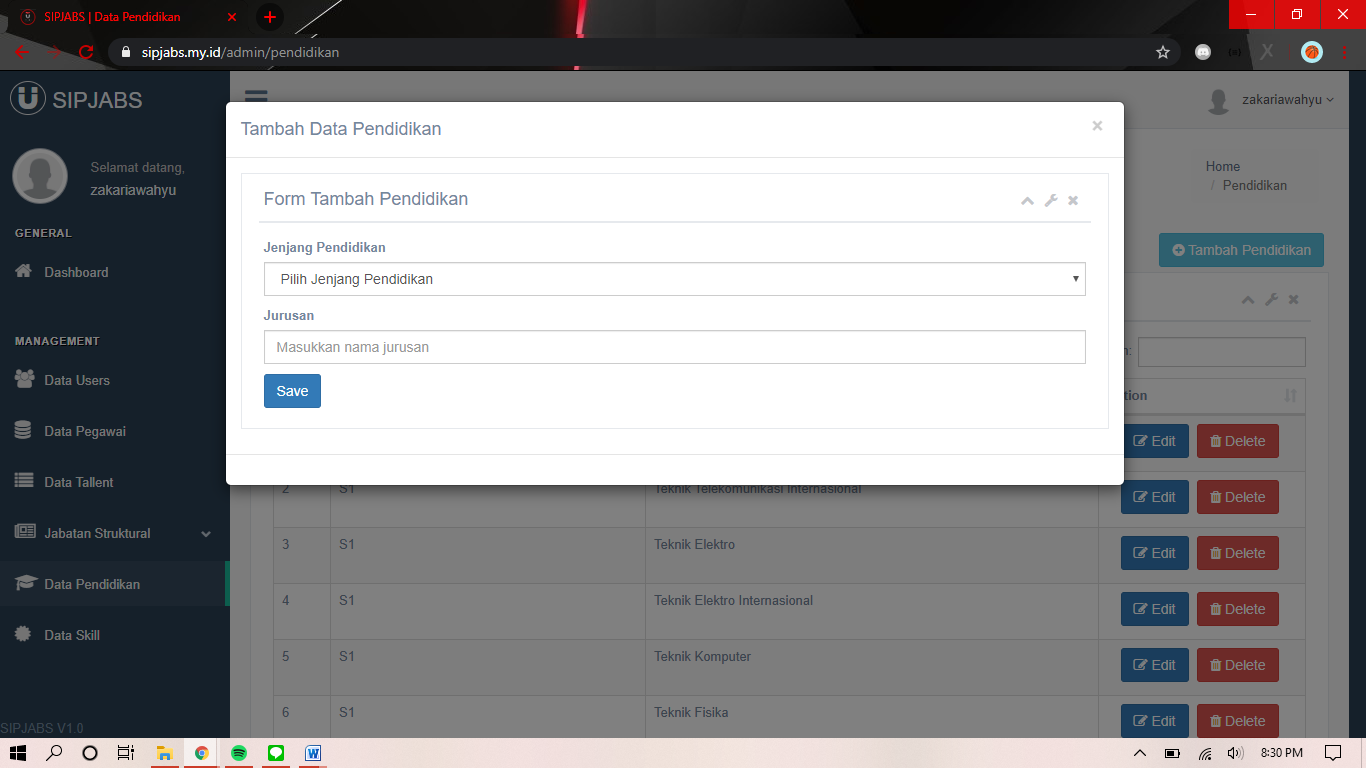
\includegraphics[width=0.8\textwidth]
		{pics/admin/implementasi/tambahpendidikan.png}
		\caption{Halaman Tambah Pendidikan - Admin}
		\label{fig:CC10}
	\end{figure}
	Gambar diatas menampilkan \textit{pop-up} tambah data pendidikan, apabila terdapat pegawai baru, namun data pendidikan belum terdaftar maka admin dapat menambahkannya dengan memilih jenjang pendidikan dan menginput jurusan,  kemudian diakhiri dengan mengklik \textit{button “save”} dan data akan tersimpan.
	
	\item Halaman Data \textit{Skill}
	\begin{figure}
		\centering
		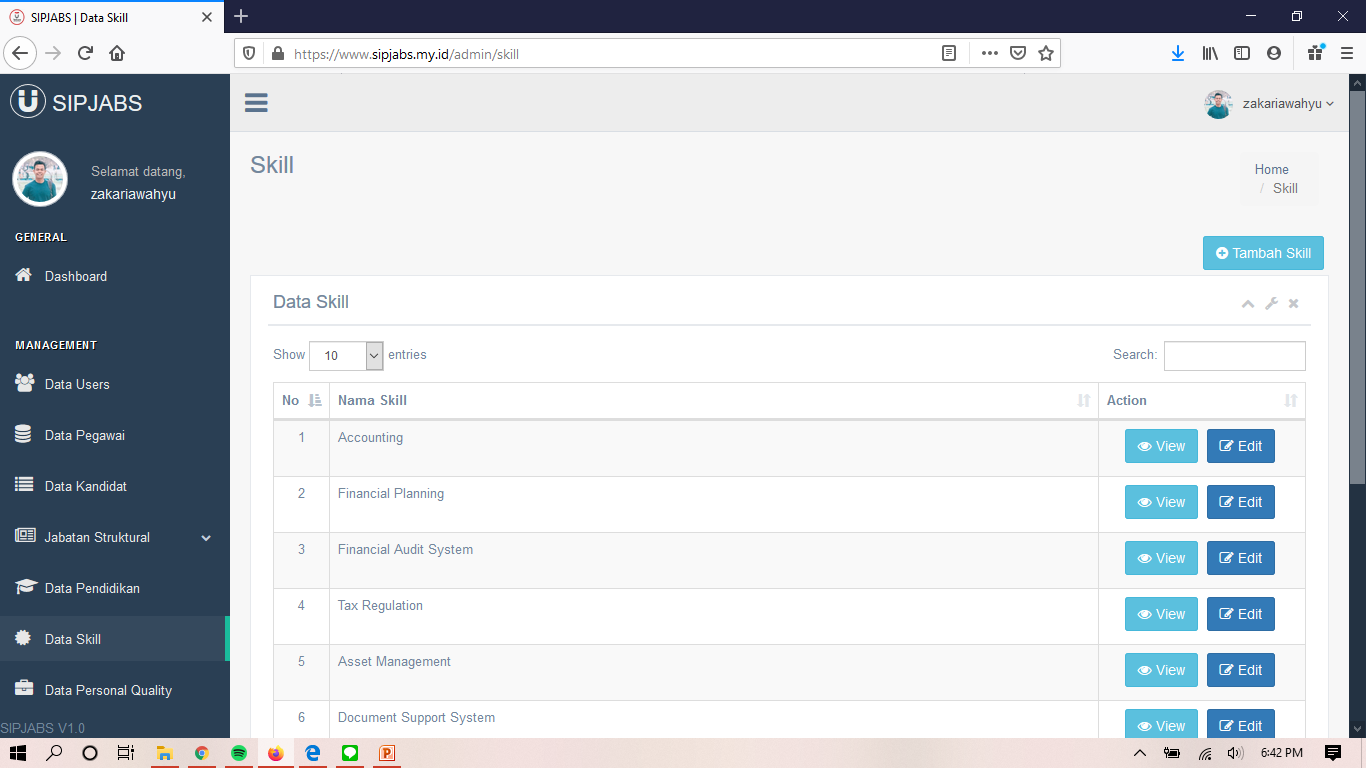
\includegraphics[width=0.8\textwidth]
		{pics/admin/implementasi/dataskill.png}
		\caption{Halaman Data \textit{Skill} - Admin}
		\label{fig:CC10}
	\end{figure}
	Gambar diatas merupakan implementasi data \textit{skill} yang ada di Universitas Telkom, data tersebut ada karena setiap pegawai memiliki \textit{skill} kemudian data \textit{skill} dari semua pegawai disatukan didalam data \textit{skill},  untuk menunjang pekerjaan. 
	
	\item Halaman \textit{Edit Skill}
	\begin{figure}
		\centering
		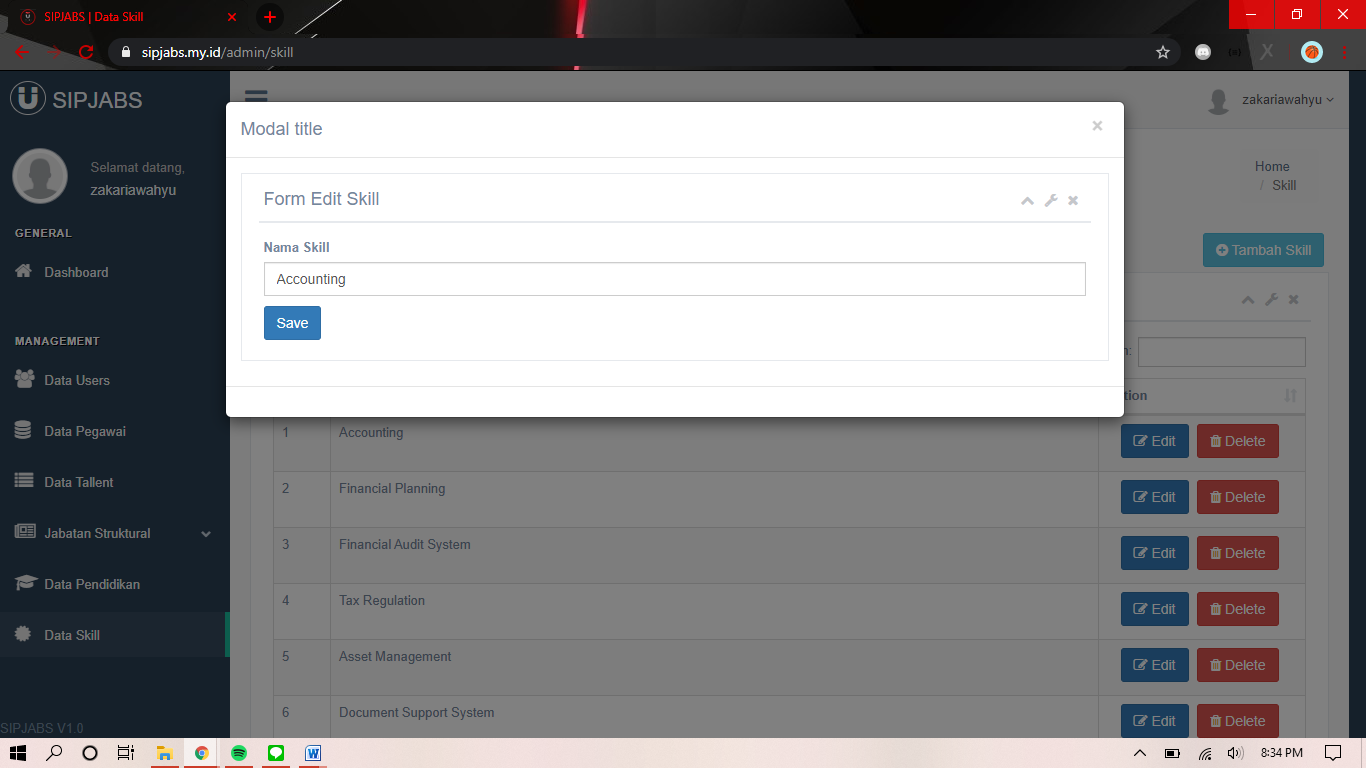
\includegraphics[width=0.8\textwidth]
		{pics/admin/implementasi/editskill.png}
		\caption{Halaman \textit{Edit Skill} - Admin}
		\label{fig:CC10}
	\end{figure}
	Implementasi diatas menampikan \textit{pop-up form edit skill}, dimana admin dapat mengedit nama \textit{skill} menjadi lebih sesuai, dan menyimpannya kembali dengan mengklik \textit{button “save”}.
	
	\item Halaman Tambah Skill
	\begin{figure}
		\centering
		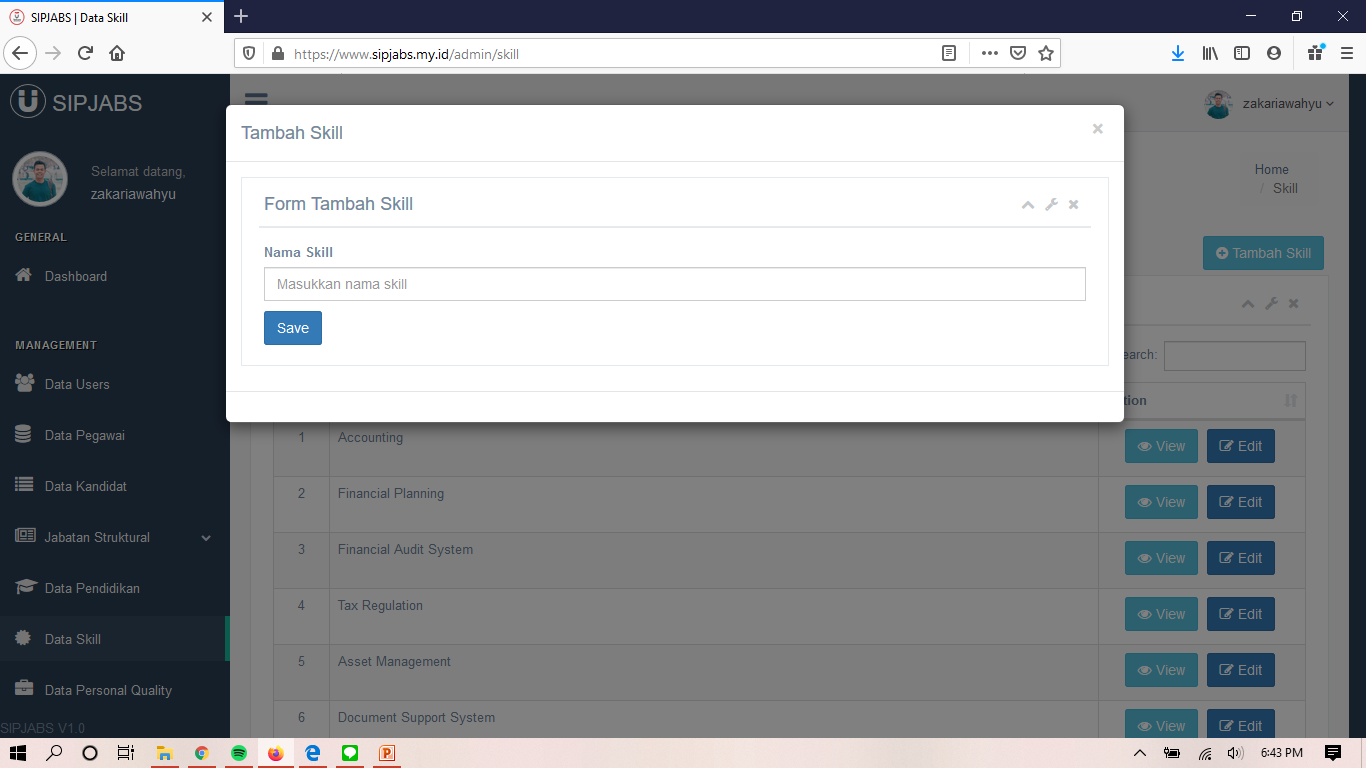
\includegraphics[width=0.8\textwidth]
		{pics/admin/implementasi/tambahskill.png}
		\caption{Halaman Tambah Skill - Admin}
		\label{fig:CC10}
	\end{figure}
	Untuk tampilan diatas adalah tambah data \textit{skill}, admin dapat menambahkan data \textit{skill} dengan mengkil button “tambah \textit{skill}” apabila \textit{skill} pada pegawai belum terdaftar pada data \textit{skill}, lalu inputkan nama \textit{skill} dan menyimpannya dengan klik \textit{button “save”}.
	
\end{enumerate}

\subsection{Implementasi \textit{User}}

\begin{enumerate}
	
	\item Halaman \textit{Login}
	\begin{figure}
		\centering
		\includegraphics[width=0.8\textwidth]
		{pics/user/implementasi/login.png}
		\caption{Halaman \textit{Login User}}
		\label{fig:CC10}
	\end{figure}
	
	Tampilan diatas merupakan implementasi dari BAB III dimana \textit{user} harus menginputkan \textit{username} dan \textit{password} untuk dapat melanjutkan penggunaan aplikasi, apabila sudah diinputkan lanjut untuk mengklik \textit{button “login”}. 
	
	\item Halaman \textit{Dashboard}
	\begin{figure}
		\centering
		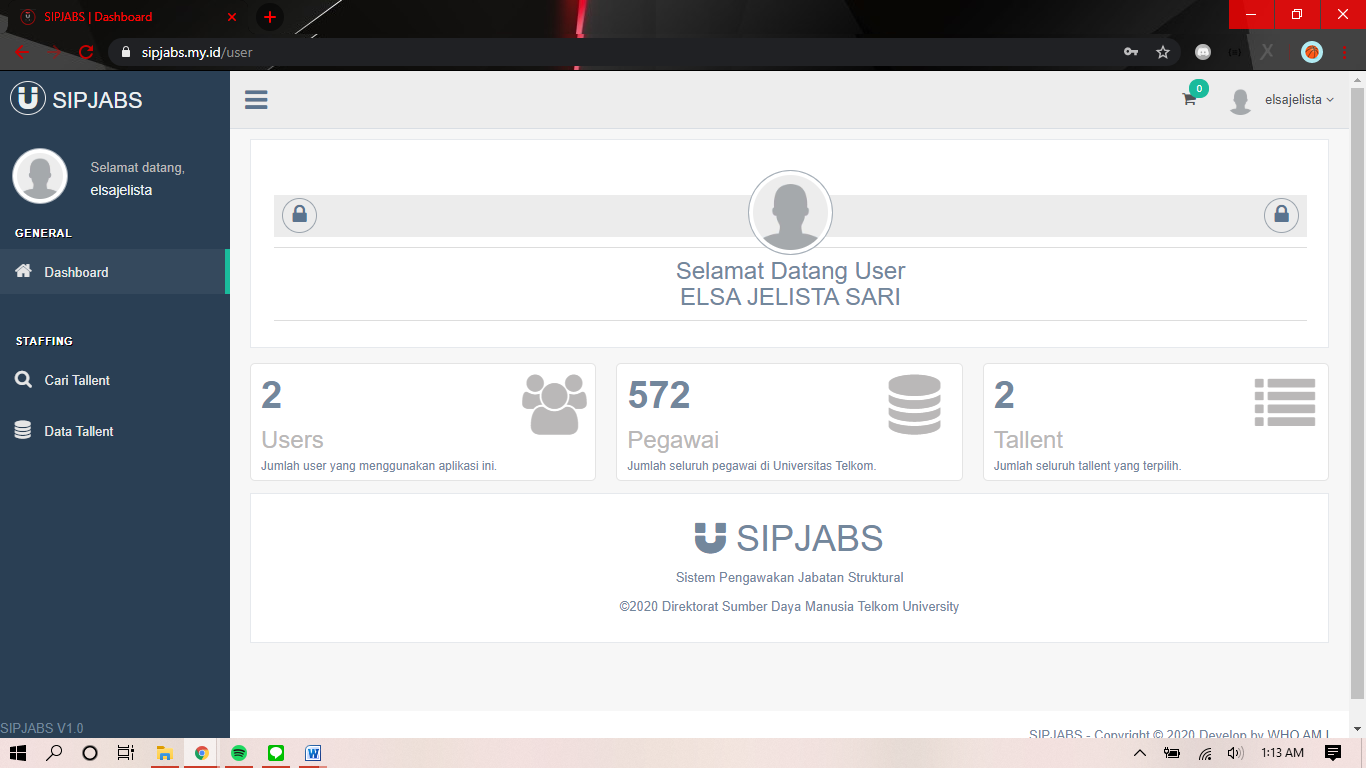
\includegraphics[width=0.8\textwidth]
		{pics/user/implementasi/dashboard.png}
		\caption{Halaman \textit{Dashboard User}}
		\label{fig:CC10}
	\end{figure}
	
	Gambar diatas mengimplementasikan isi dari \textit{dashboard user}, berbeda dengan \textit{dashboard} yang dimiliki admin, \textit{dashboard user} hanya menampilkan jumlah \textit{user} yang dapat mengakses aplikasi \textbf{SiPJabS}, jumlah pegawai yang terdaftar di Universitas Telkom, serta jumlah \textit{tallent} yang sudah dipilih. 
	
	\item Halaman \textit{Profile}
	\begin{figure}
		\centering
		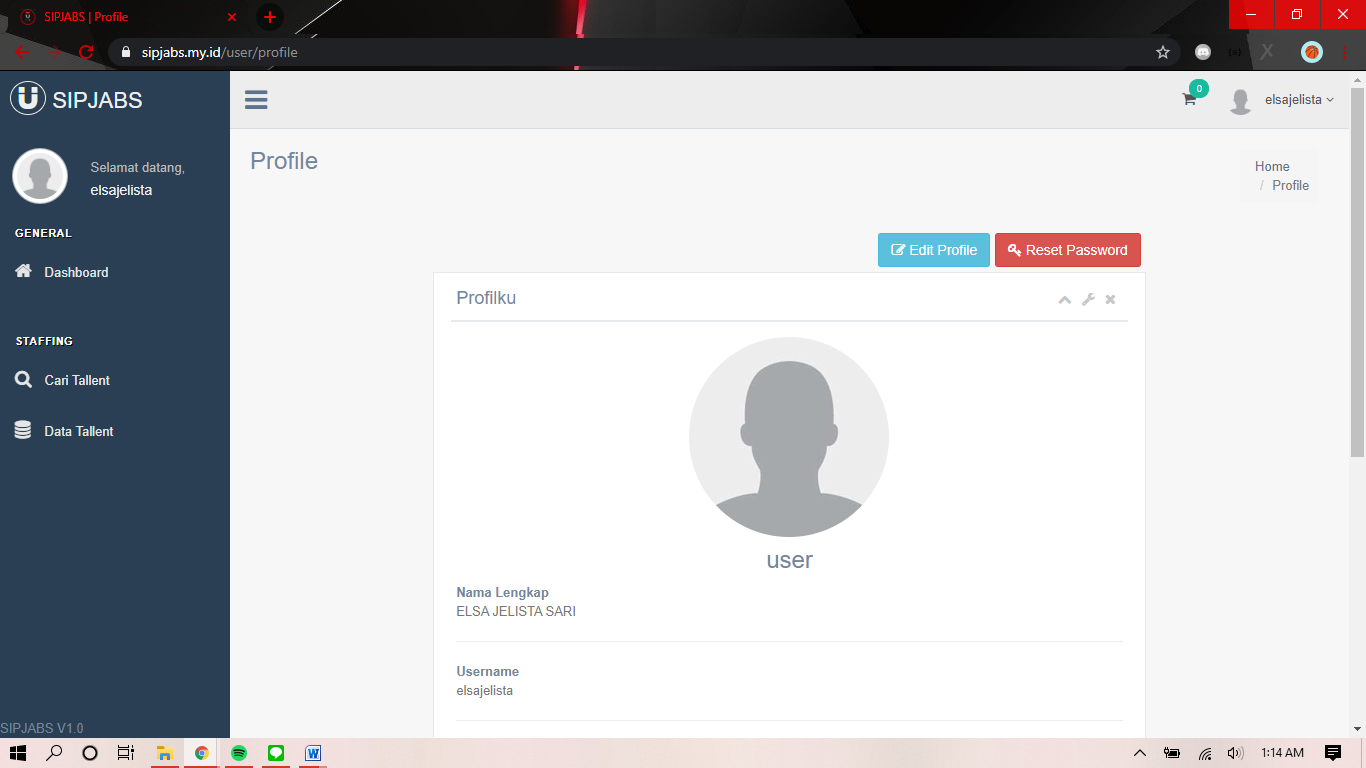
\includegraphics[width=0.8\textwidth]
		{pics/user/implementasi/profile.png}
		\caption{Halaman \textit{Profile User}}
		\label{fig:CC10}
	\end{figure}
	
	Implementasi diatas menunjukkan isi \textit{profile} dari \textit{user}, terdapat nama lengkap, \textit{username}, email, status pegawai, unit kerja, jabatan, dan NIP. Admin dapat membuka halaman tersebut dengan cara klik \textit{username} yang ada di atas kanan, kemudian akan terdapat \textit{dropdown} dan klik \textit{profile}, maka halaman akan tampil seperti diatas. 
	
	\item Halaman \textit{Edit Profile}
	\begin{figure}
		\centering
		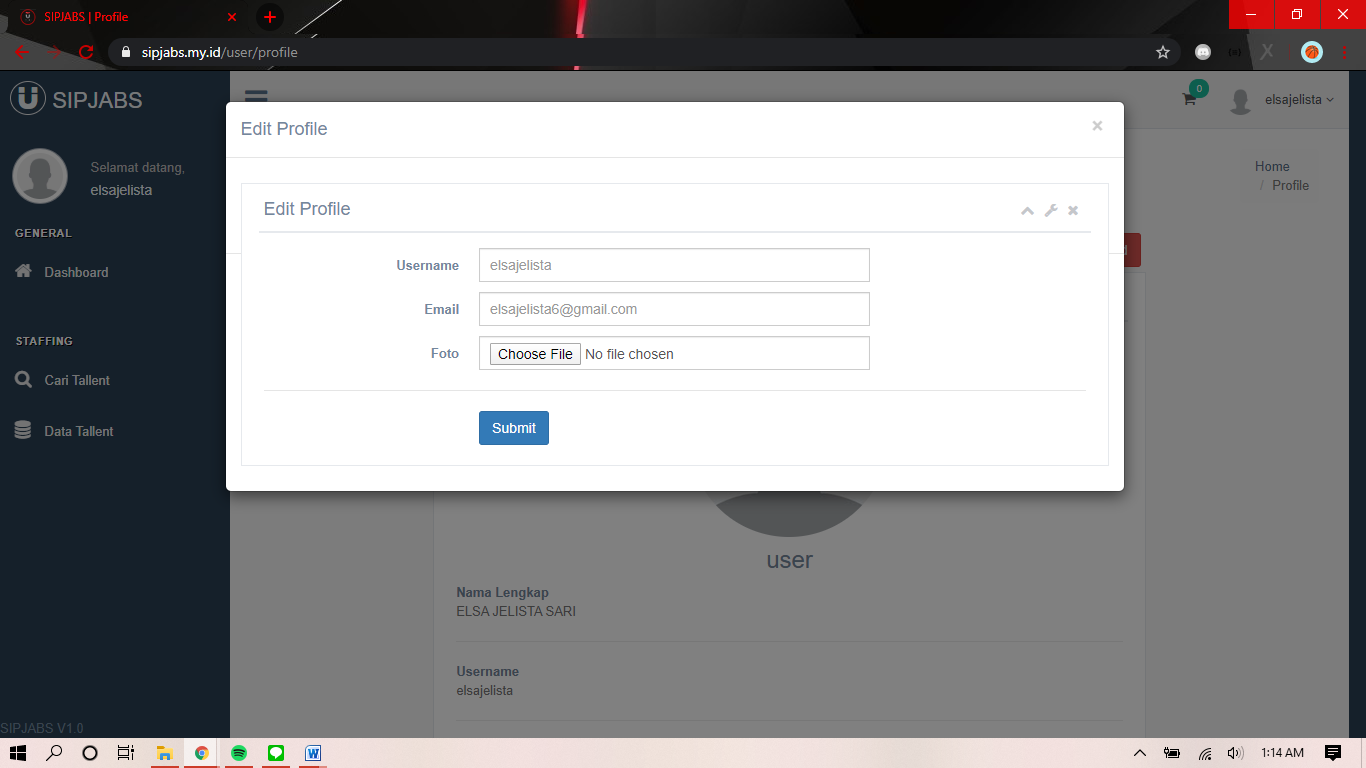
\includegraphics[width=0.8\textwidth]
		{pics/user/implementasi/editprofile.png}
		\caption{Halaman \textit{Edit Profile User}}
		\label{fig:CC10}
	\end{figure}
	
	Gambar diatas mengimplementasikan\textit{ edit profile user} dengan \textit{pop-up}, \textit{user} dapat mengganti \textit{username}, email atau foto. Kemudian klik “\textit{submit}” untuk menyimpan data yang sudah diganti agar tersimpan.
	
	\item Halaman \textit{Reset Password}
	\begin{figure}
		\centering
		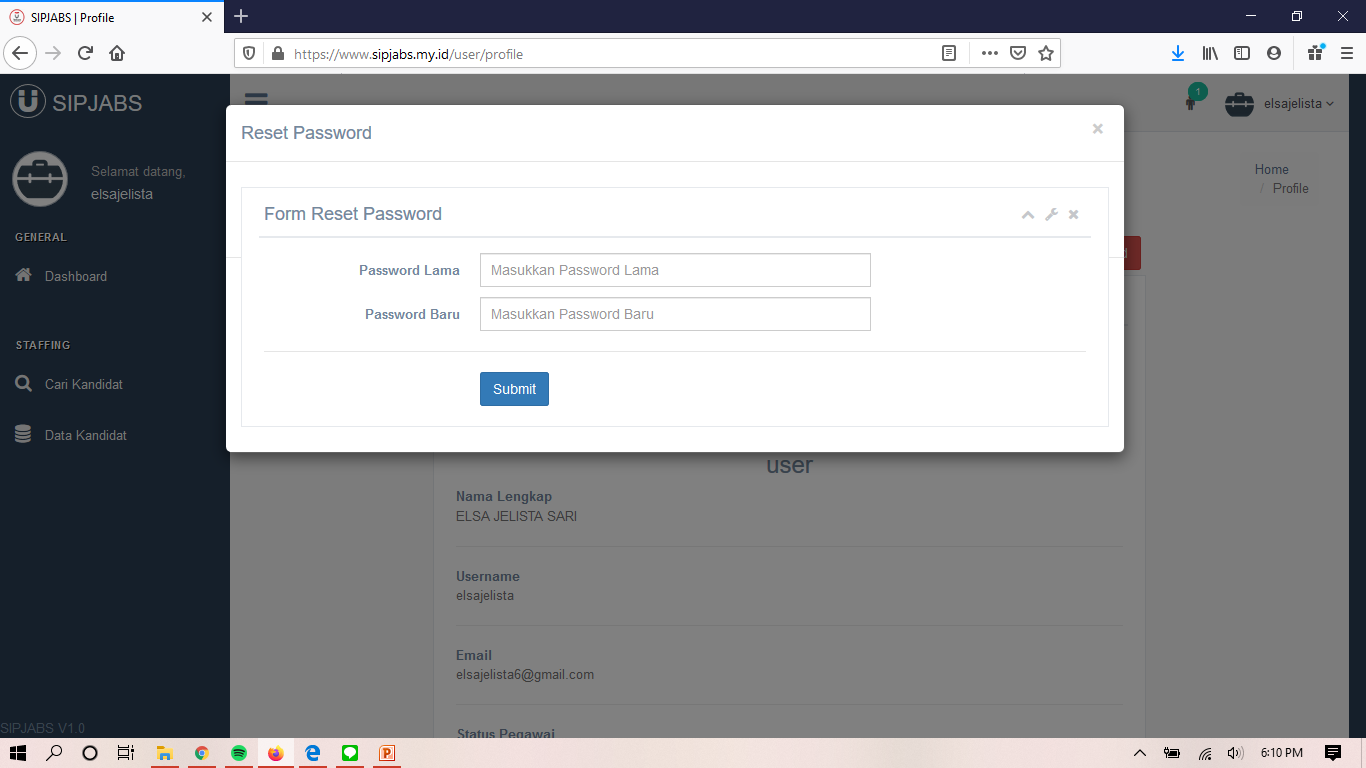
\includegraphics[width=0.8\textwidth]
		{pics/user/implementasi/resetpassword.png}
		\caption{Halaman \textit{Reset Password User}}
		\label{fig:CC10}
	\end{figure}
	
	Implementasi diatas menjelaskan bahwasannya \textit{user} dapat mengganti \textit{passsword}, apabila \textit{password} tersebut sudah diketahui oleh pihak lain, \textit{user} dapat mengklik \textit{button “reset password”} kemudian akan tampil\textit{ pop-up} seperti diatas, \textit{user} harus menginputkan \textit{password} lama dan \textit{password} yang baru, lalu klik “\textit{submit}” untuk menyimpan \textit{password} yang baru.
	
	\item Halaman \textit{Help}
	\begin{figure}
		\centering
		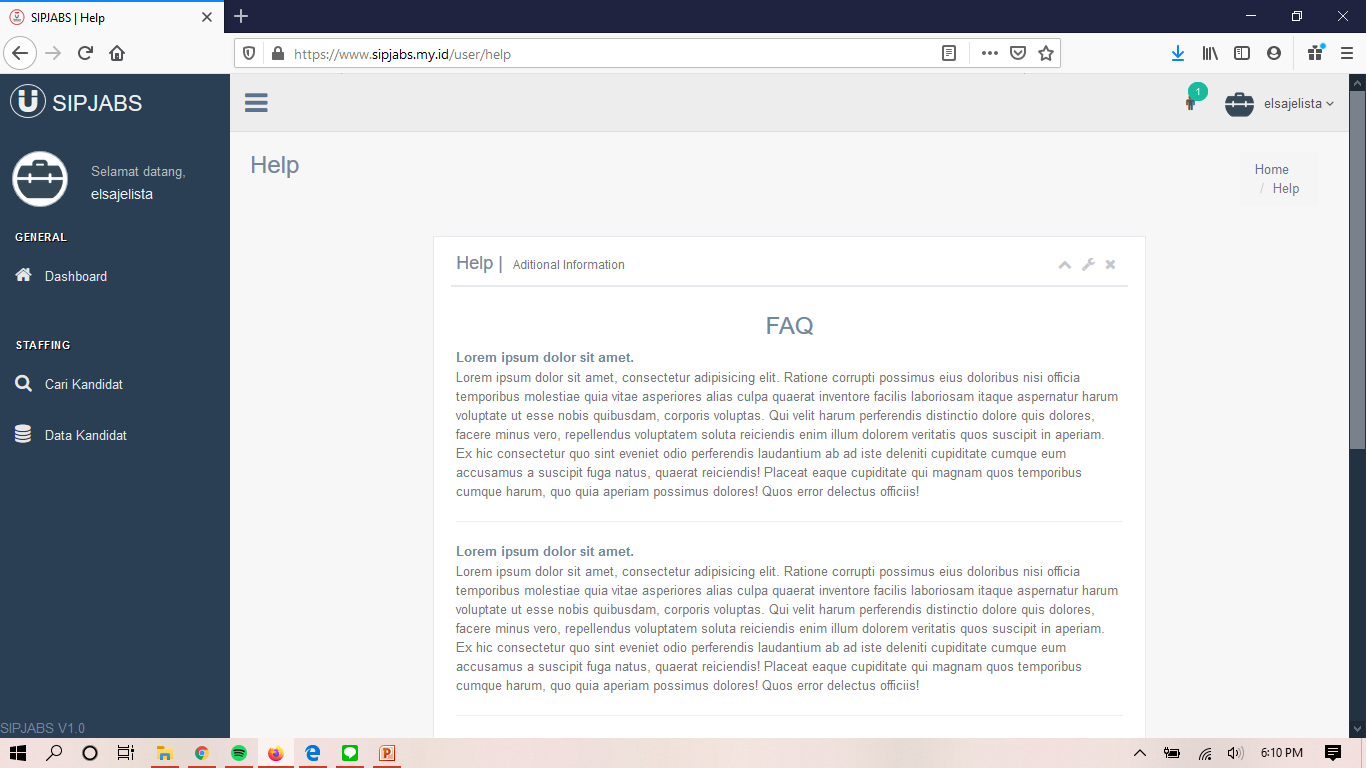
\includegraphics[width=0.8\textwidth]
		{pics/user/implementasi/help.png}
		\caption{Halaman \textit{Help User}}
		\label{fig:CC10}
	\end{figure}

	\newpage
	\item Halaman Cari \textit{Tallent}
	\begin{figure}
		\centering
		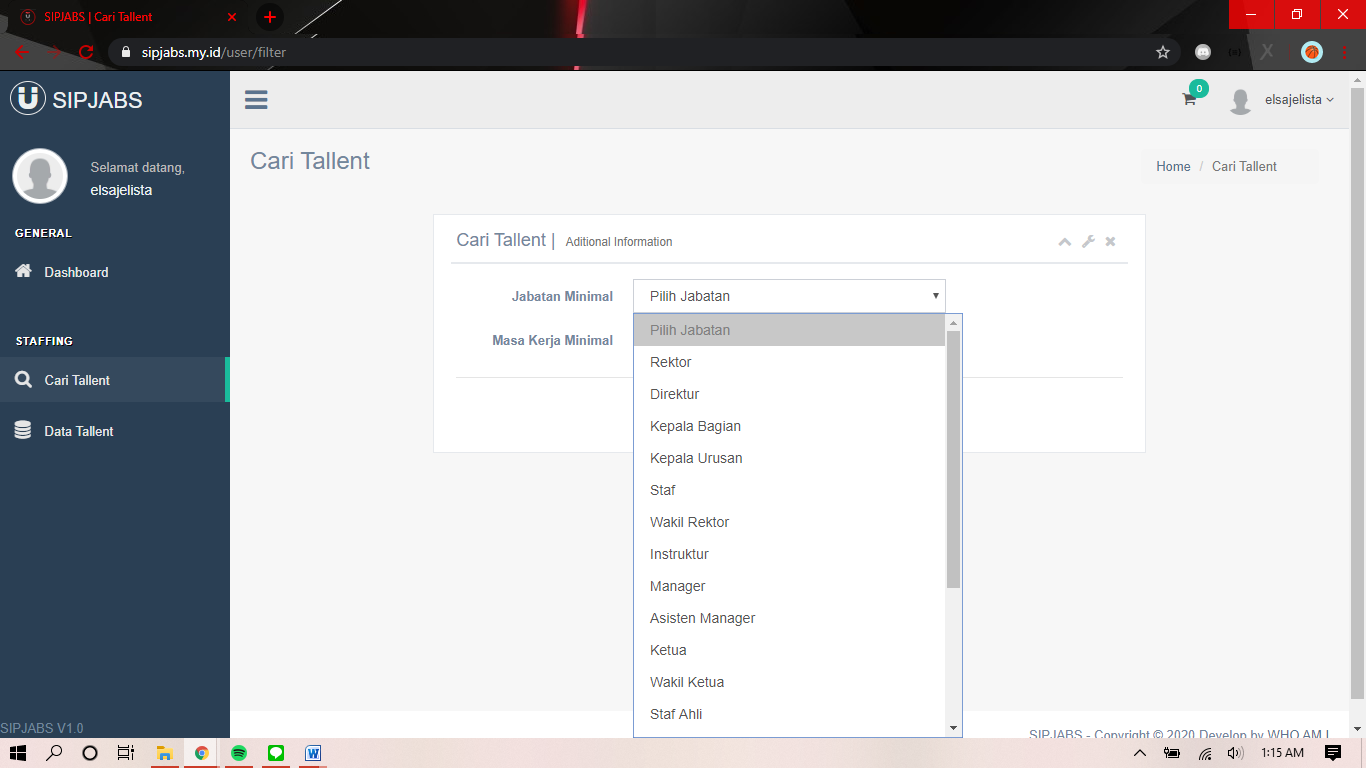
\includegraphics[width=0.8\textwidth]
		{pics/user/implementasi/caritallent.png}
		\caption{Halaman Cari \textit{Tallent - User}}
		\label{fig:CC10}
	\end{figure}
	
	Gambar diatas mengimplementasikan apabila \textit{user} ingin mencari \textit{tallent} yang dibutuhkan sesuai \textit{requirement} perusahaan untuk menggantikan atau mengisi posisi yang kosong, dengan cara klik “cari tallent” pada menu, lalu akan muncul halaman seperti diatas, user harus memilih jabatan minimal yang dibutuhkan dan menginputkan masa kerja. Dan klik \textit{button} “cari” untuk mencari \textit{tallent}.
	
	\item Halaman \textit{Filtering}
	\begin{figure}
		\centering
		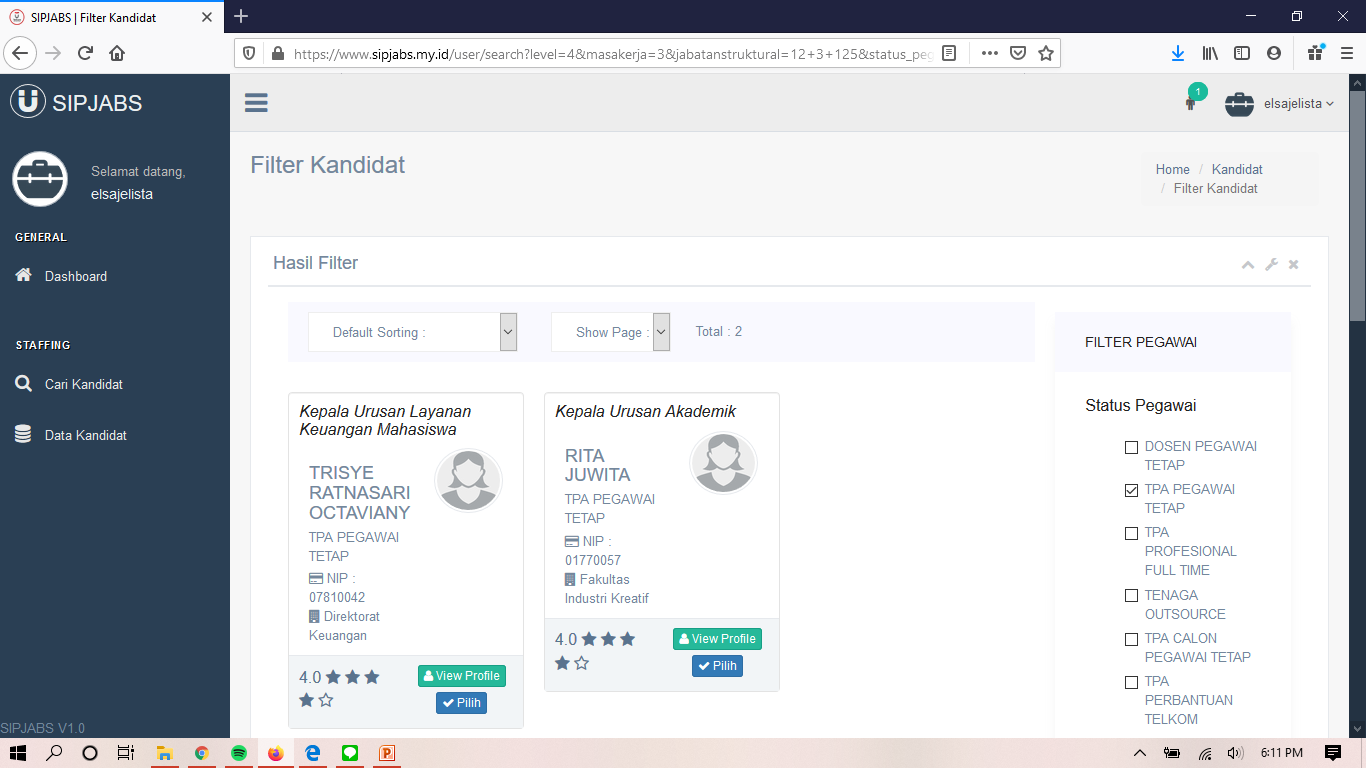
\includegraphics[width=0.8\textwidth]
		{pics/user/implementasi/hasiltallent.png}
		\caption{Halaman \textit{Filtering - User}}
		\label{fig:CC10}
	\end{figure}
	
	Implementasi diatas menampilkan data \textit{tallent} yang tersedia, kemudian \textit{user} dapat menyeleksi kembali dengan memilih \textit{filter} pegawai, jenjang pendidikan, jurusan dan \textit{skill} yang dimiliki oleh pegawai.
	
	\item Halaman\textit{ View Detail} Pegawai
	\begin{figure}
		\centering
		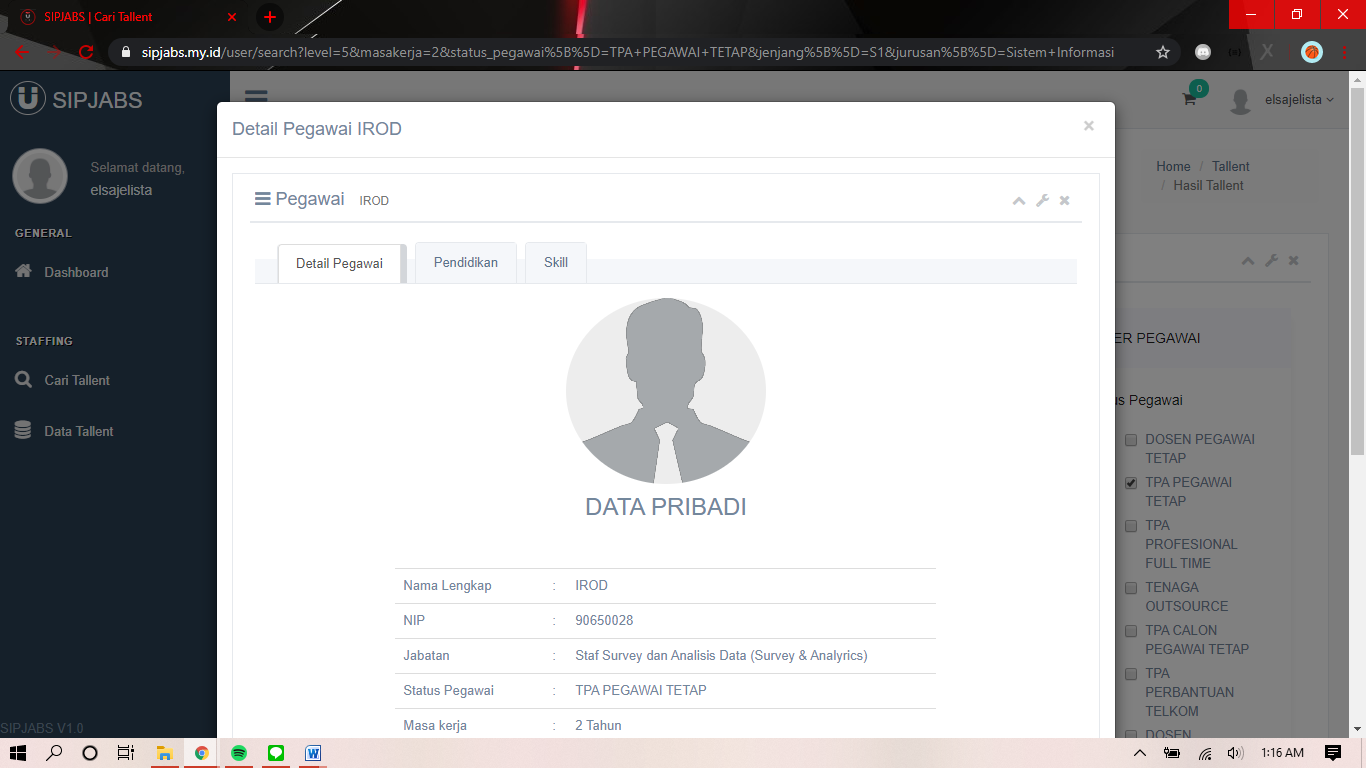
\includegraphics[width=0.8\textwidth]
		{pics/user/implementasi/viewdetailpegawai.png}
		\caption{Halaman \textit{View Detail} Pegawai - \textit{User}}
		\label{fig:CC10}
	\end{figure}
	
	Gambar diatas mengimpementasikan bahwasannya \textit{user} dapat melihat data pribadi yang dimiliki \textit{tallent}, dengan cara klik\textit{ button “view”} maka akan tampil halaman seperti diatas
	
	\item Halaman \textit{Cart}
	\begin{figure}
		\centering
		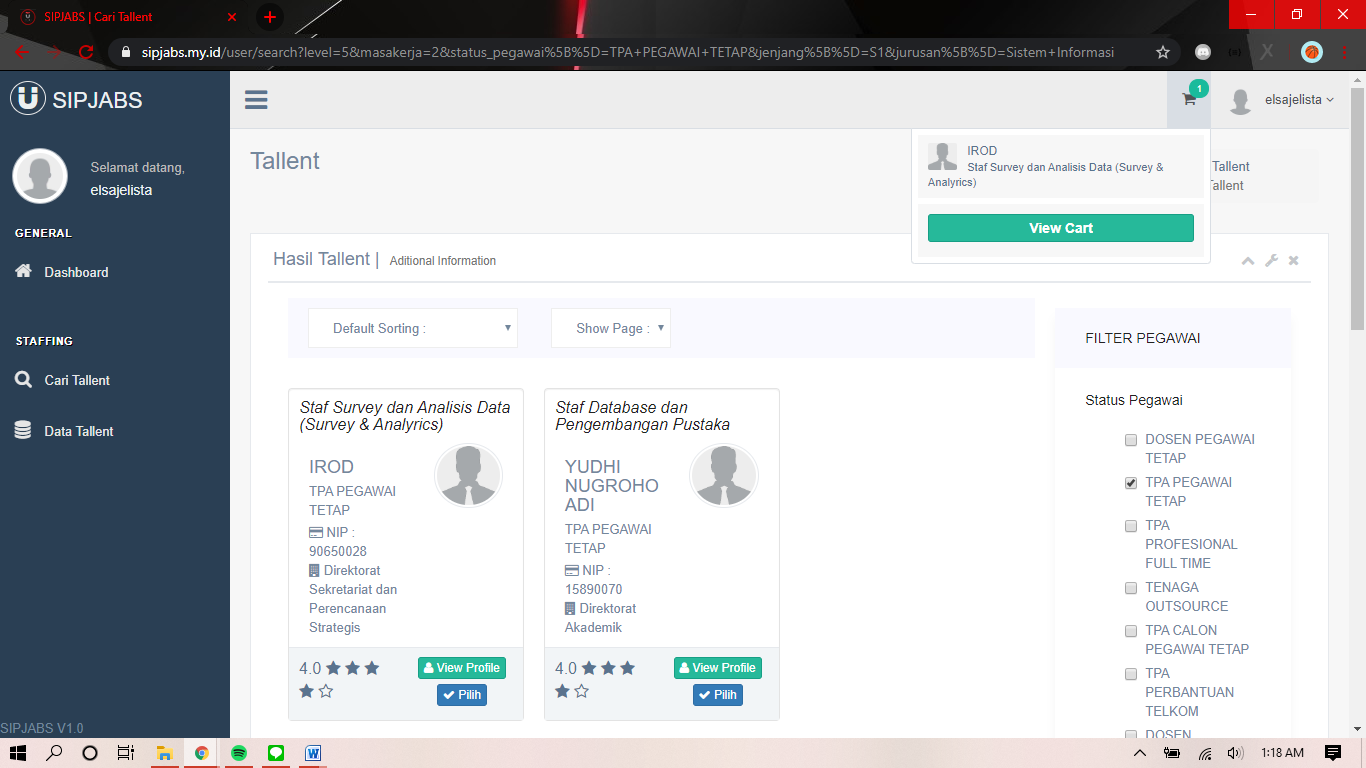
\includegraphics[width=0.8\textwidth]
		{pics/user/implementasi/cartuser.png}
		\caption{Halaman \textit{Cart - User}}
		\label{fig:CC10}
	\end{figure}
	
	Gambar diatas menjelaskan bahwasannya \textit{user} sudah memilih \textit{tallent} yang sesuai dengan yang dibutuhkan untuk mengganti atau mengisi posisi yang kosong.  
	
	\newpage
	\item Halaman \textit{View Cart}
	\begin{figure}
		\centering
		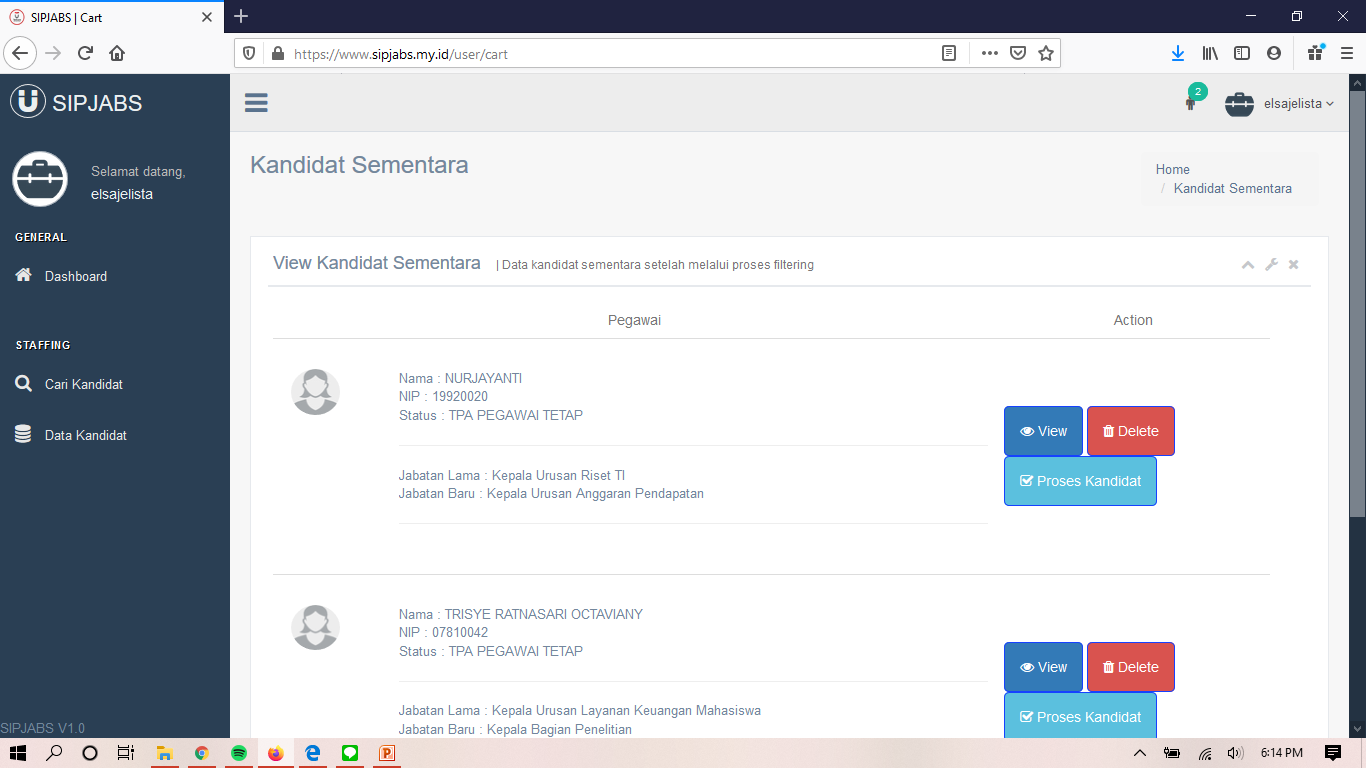
\includegraphics[width=0.8\textwidth]
		{pics/user/implementasi/viewcart.png}
		\caption{Halaman \textit{View Cart - User}}
		\label{fig:CC10}
	\end{figure}
	
	Gambar diatas mengimplementasikan halaman \textit{view }pada \textit{cart}, apabila \textit{user} telah memilih \textit{tallent} maka data tersebut akan masuk kedalam \textit{cart}, sebelum diproses ke data tallent. 
	
		\item Halaman Data \textit{Tallent}
	\begin{figure}
		\centering
		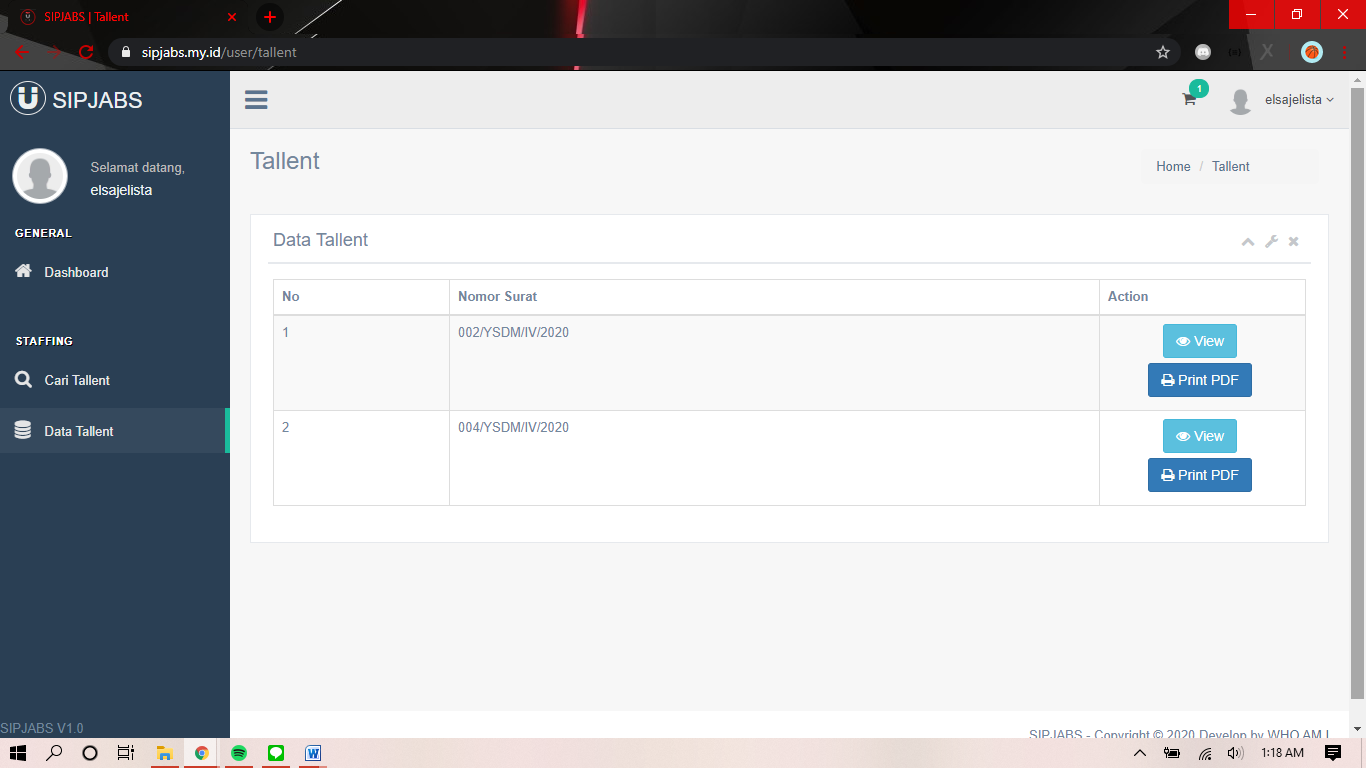
\includegraphics[width=0.8\textwidth]
		{pics/user/implementasi/datatallent.png}
		\caption{Halaman Data \textit{Tallent - User}}
		\label{fig:CC10}
	\end{figure}
	
	Gambar diatas mengimplementasikan isi dari  data \textit{tallent} yang dimiliki \textit{user}, data tersebut sudah dipilih sesuai dengan \textit{requirement} perusahaan dan sesuai dengan \textit{job descripton} yang dimiliki pegawai.
	
\end{enumerate}


 


%-----------------------------------------------------------------------------%
\section{Pengujian Aplikasi}
%-----------------------------------------------------------------------------%
\blindtext \\

\begin{figure}
	\centering
	\begin{tabular}[c]{cc}
		
		\begin{subfigure}[t]{0.45\textwidth}
			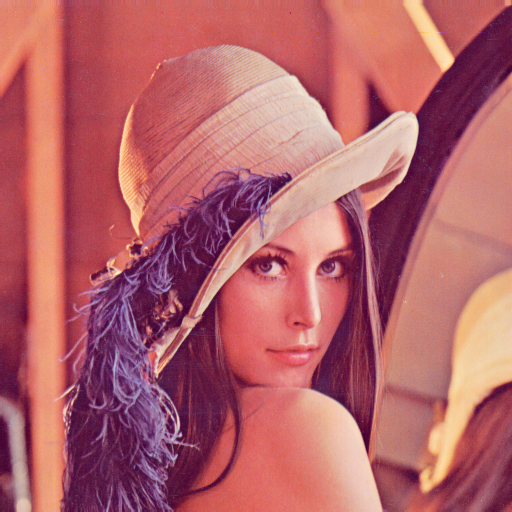
\includegraphics[width=\linewidth]{pics/lena.png}
			\caption{Testing With Lena} \label{fig:4a}
		\end{subfigure}
		\hspace*{\fill} % separation between the subfigures
		
		\begin{subfigure}[t]{0.45\textwidth}
			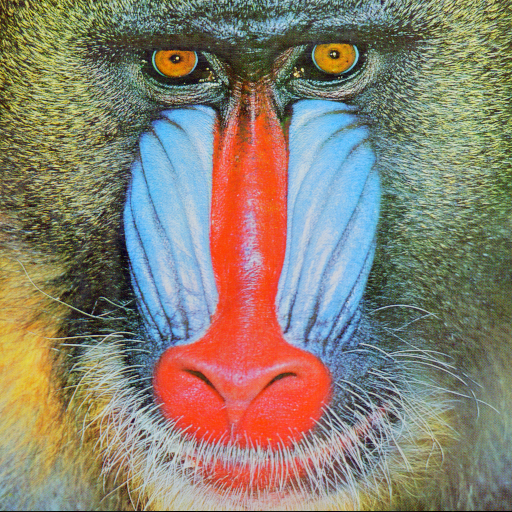
\includegraphics[width=\linewidth]{pics/baboon.png}
			\caption{Testing With Baboon} \label{fig:4b}
		\end{subfigure}
		
	\end{tabular}
	\caption{Pengujian Gambar Pada Aplikasi Z}
	\label{fig:41}
\end{figure}

%-----------------------------------------------------------------------------%
\subsection{Pengujian Alpha}
%-----------------------------------------------------------------------------%

\blindtext \\



\subsection{Pengujian Fungsionalitas}
\blindtext \\

\subsection{Pengujian Kesesuaian}
\blindtext \\

%-----------------------------------------------------------------------------%
\subsection{Pengujian Beta}
%-----------------------------------------------------------------------------%

\blindtext \\


%-----------------------------------------------------------------------------%
\section{Diskusi Hasil Pengujian}
%-----------------------------------------------------------------------------%

\begin{figure}
	\centering
	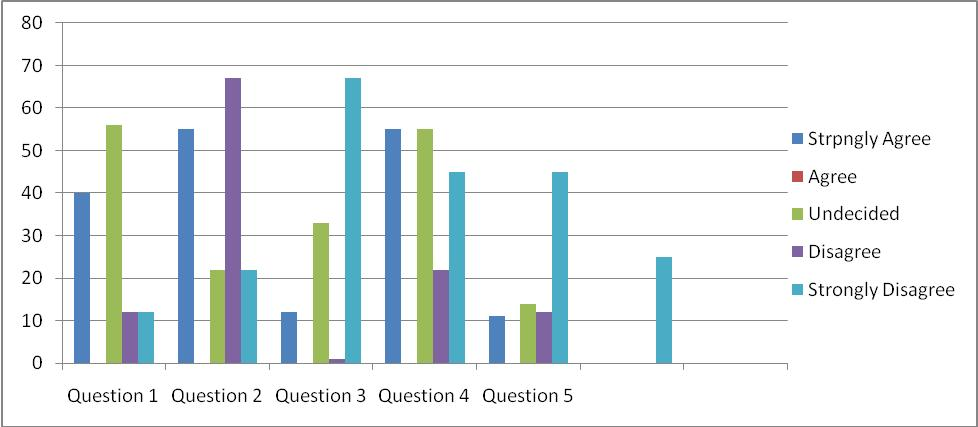
\includegraphics[width=0.8\textwidth]
	{pics/graph1.jpg}
	\caption{My Survey Results 2020}
	\label{fig:42}
\end{figure}

\blindtext \\